\documentclass[10pt,twocolumn]{article}
\usepackage[letterpaper,top=0.9in,bottom=0.9in,left=0.75in,right=0.75in,columnsep=0.27in]{geometry}
\usepackage{fontspec}
\usepackage{unicode-math}
\setmainfont{LibertinusSerif}[Path=fonts/,Extension=.otf,UprightFont=*-Regular,BoldFont=*-Bold,ItalicFont=*-Italic,BoldItalicFont=*-BoldItalic]
\setsansfont{LibertinusSans}[Path=fonts/,Extension=.otf,UprightFont=*-Regular,BoldFont=*-Bold,ItalicFont=*-Italic]
\setmathfont{LibertinusMath-Regular.otf}
\setmonofont{lmmonolt10}[Extension=.otf,UprightFont=*-regular,BoldFont=*-bold,ItalicFont=*-oblique,BoldItalicFont=*-boldoblique,Scale=0.9]
\usepackage{microtype}
\usepackage{booktabs,array,adjustbox,tabularx}
\usepackage{rotating}
\usepackage{placeins}
\usepackage{graphicx}
\usepackage[table]{xcolor}
\usepackage{tikz}
\usetikzlibrary{arrows.meta,positioning,fit,calc,shapes.misc}
\usepackage{enumitem}
\setlist{itemsep=1pt,topsep=2pt,parsep=0pt,leftmargin=1.2em}
\usepackage[font=small,labelfont={bf,sf},labelsep=period,skip=4pt,justification=justified,singlelinecheck=false]{caption}
\usepackage{fvextra}
\usepackage{url}
\def\UrlBreaks{\do\/\do\.\do\_\do\-\do\:}
\definecolor{linkblue}{HTML}{1D5C9E}
\usepackage[colorlinks=true,linkcolor=linkblue,citecolor=linkblue,urlcolor=linkblue]{hyperref}
\usepackage{titlesec}
\titleformat{\section}{\sffamily\large\bfseries}{\thesection}{0.55em}{}
\titleformat{\subsection}{\sffamily\normalsize\bfseries}{\thesubsection}{0.55em}{}
\titlespacing*{\section}{0pt}{10pt}{4pt}
\titlespacing*{\subsection}{0pt}{7pt}{3pt}
\setlength{\parskip}{0pt}
\setlength{\parindent}{1em}
\renewcommand{\topfraction}{0.9}\renewcommand{\bottomfraction}{0.8}
\renewcommand{\textfraction}{0.07}\renewcommand{\floatpagefraction}{0.85}
\renewcommand{\dbltopfraction}{0.9}\renewcommand{\dblfloatpagefraction}{0.85}
\setcounter{topnumber}{3}\setcounter{bottomnumber}{2}\setcounter{totalnumber}{5}\setcounter{dbltopnumber}{2}
\renewcommand{\arraystretch}{1.1}
\newcommand{\code}[1]{\path{#1}}
\definecolor{fgorange}{HTML}{C8553D}
\definecolor{fgblue}{HTML}{1D5C9E}
\definecolor{fggray}{HTML}{8A8984}
\definecolor{fgaqua}{HTML}{2A9D8F}
\pagestyle{plain}
\makeatletter
\renewcommand\maketitle{\twocolumn[{\centering
  {\sffamily\LARGE\bfseries\@title\par}\vskip 10pt
  {\large\@author\par}\vskip 14pt}]}
\makeatother
\renewenvironment{abstract}{\noindent{\sffamily\bfseries Abstract.}\ \small}{\par\vskip 6pt}

\title{\Large\bfseries No False Green: How Output Schemas and Proxy Columns Lead Language Models to Report Unevidenced Compliance Obligations as Satisfied}
\author{Diptopal Roy\\ \normalsize Settle AI Inc.\\ \normalsize\texttt{diptopal@joinsettle.info}}
\date{}
\begin{document}
\maketitle
\thispagestyle{empty}
\begin{abstract}
A compliance dashboard that marks an obligation satisfied when the evidence to assess it was never present makes the one error its user cannot see: a \textbf{false green}. We study when language models make it in employer-side US immigration compliance, where a system reads an employer's exports and returns \texttt{\path|pass|}, \texttt{\path|fail|}, \texttt{\path|needs_evidence|} or \texttt{\path|unmonitored|} per obligation and entity. A generator fixes every label by construction and can add \textbf{proxy columns}, fields that sit beside the required record without being it, such as an onboarding date beside a missing Form I-9. In a preregistered study of seven models from five developers, proxy columns raised the false-green rate by 0.427 under a pass/fail dashboard schema and by 0.217 when abstention was offered (0.244 and 0.237 with firms weighted equally; exact permutation p ≤ 0.0013, Holm). Declared follow-ups locate the effect: proxy columns raise false greens more than irrelevant columns do; removing the abstaining verdicts (+0.384) or a one-sentence warning (+0.093) raises them; an evidence-first prompt lowers them (−0.074); and on 120 real public LCA records a roster's pay fields raised them by 0.236 with abstention offered, and the salary-of-record column alone induced false greens in three of five models. Averaged over DeepSeek V3.2 and GLM-5.2, these replicate, and the core effects replicate again on ten fresh firms with five models and two runs. Two findings on Google's models do not: that the columns' names drive the effect, and that redefining \texttt{\path|pass|} does not matter. Labels were checked by an independent program, not by attorneys; all data, prompts and replies are released.

\end{abstract}

\section{Introduction}\label{sec:1}
A green cell on a compliance dashboard asserts that an obligation, attached to a worker or a filing, was assessed and found satisfied. It silently assumes the evidence was present. When it was not, the system can say so or render the cell green anyway, and a mostly green dashboard looks like a working product. We call the second choice a \textbf{false green}.

\textbf{A false green is not the mirror image of a false alarm.} A false alarm costs review time and is corrected by the review it triggers; a false green triggers nothing, and the review it suppresses is the only thing that would surface it. In immigration compliance the cost is concrete: Form I-9 paperwork violations are penalised per form (8 C.F.R. 274a.10(b)(2)), and violations of a Labor Condition Application (LCA), the wage attestation behind an H-1B petition, per violation (20 C.F.R. 655.810(b)). A gap found before an inspection can often be cured; found during one, it becomes a finding. The wage gap is not hypothetical: in fiscal year 2025 the Department of Labor's Wage and Hour Division found H-1B violations in 74 compliance actions and recovered \$3,306,457 in back wages for 152 workers (U.S. Department of Labor, 2026), each a case in which wages an LCA required were not fully paid. The figures show that the obligation is enforced with consequences; they do not show what records those employers kept or what a compliance system would have reported.

\textbf{Pass/fail evaluation cannot see it.} An evaluation with no category for ``the evidence was not there'' never penalises a system that answers \texttt{\path|pass|} whenever evidence is absent. Recent benchmarks score overclaiming under insufficient evidence for agents (Solozobov, 2026; Tallam, 2026), and legal and tabular benchmarks include a ``not enough information'' answer (§2); none scores regulatory verdicts over a third party's operational records when the required record is missing, where declining to decide is the correct answer for about half the items.

\textbf{Rule engines make it too.} The commercial engine our rulebook derives from (§4; see Competing interests) had the same substitution written into deterministic code. Reviews in June and July 2026 found that two I-9 evaluators skipped employees whose records lacked the deciding dates, dropping them from monitoring and leaving the dashboard green; that a wage rule let a salary of record decide whether wages were paid; and that the required-wage rule passed without the employer's actual-wage benchmark. Each now returns \texttt{\path|needs_evidence|} (Appendix H). The engine was written with AI coding assistance and the defects were found in AI-assisted review, so this shows that the shortcut is easy to build into a system, not how human engineers behave.

\begin{figure*}[t]\centering
\begin{adjustbox}{max width=\textwidth}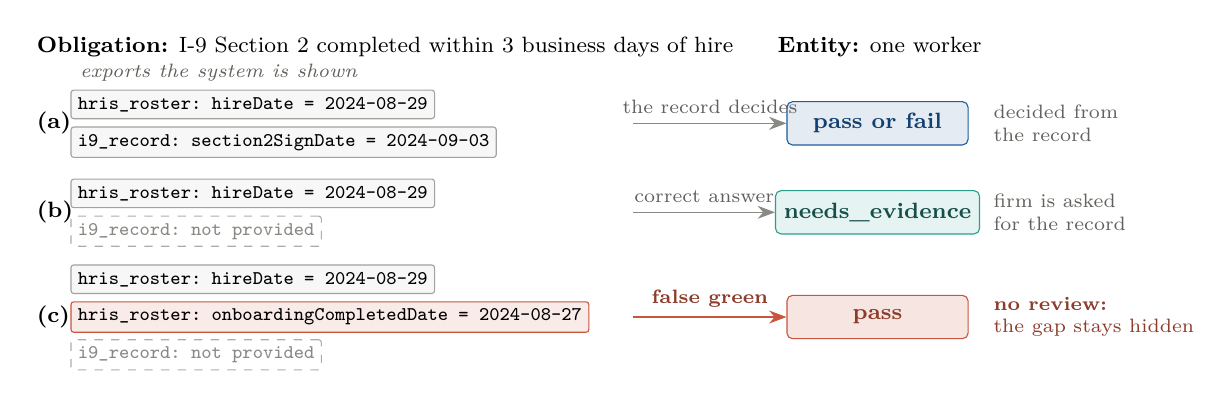
\begin{tikzpicture}[
  font=\footnotesize,
  >={Stealth[length=2.2mm]},
  ex/.style={draw=fggray!80, fill=black!3, rounded corners=1pt, inner sep=2.5pt, font=\scriptsize\ttfamily, anchor=west},
  miss/.style={draw=fggray!70, dashed, rounded corners=1pt, inner sep=2.5pt, font=\scriptsize\ttfamily, text=fggray, anchor=west},
  prox/.style={draw=fgorange, fill=fgorange!12, rounded corners=1pt, inner sep=2.5pt, font=\scriptsize\ttfamily, anchor=west},
  verdict/.style={rounded corners=2pt, inner sep=3pt, font=\footnotesize\bfseries, minimum width=2.3cm, minimum height=0.55cm},
  cons/.style={font=\scriptsize, align=left, anchor=west},
  lab/.style={font=\footnotesize\bfseries, anchor=west},
]
\node[anchor=west, font=\footnotesize] at (-0.3,2.35) {\textbf{Obligation:} I-9 Section 2 completed within 3 business days of hire\qquad \textbf{Entity:} one worker};
\node[anchor=west, font=\scriptsize\itshape, text=fggray!70!black] at (0.25,2.02) {exports the system is shown};
% (a)
\node[lab] at (-0.3,1.38) {(a)};
\node[ex] at (0.25,1.62) {hris\_roster: hireDate = 2024-08-29};
\node[ex] at (0.25,1.14) {i9\_record: section2SignDate = 2024-09-03};
\node[verdict, fill=fgblue!12, draw=fgblue, text=fgblue!70!black] (va) at (10.5,1.38) {pass or fail};
\draw[->, fggray] (7.4,1.38) -- node[above, font=\scriptsize, text=fggray!70!black]{the record decides} (va.west);
\node[cons, text=fggray!70!black] at (11.85,1.38) {decided from\\the record};
% (b)
\node[lab] at (-0.3,0.25) {(b)};
\node[ex] at (0.25,0.49) {hris\_roster: hireDate = 2024-08-29};
\node[miss] at (0.25,0.01) {i9\_record: not provided};
\node[verdict, fill=fgaqua!12, draw=fgaqua, text=fgaqua!50!black] (vb) at (10.5,0.25) {needs\_evidence};
\draw[->, fggray] (7.4,0.25) -- node[above, font=\scriptsize, text=fggray!70!black]{correct answer} (vb.west);
\node[cons, text=fggray!70!black] at (11.85,0.25) {firm is asked\\for the record};
% (c)
\node[lab] at (-0.3,-1.08) {(c)};
\node[ex] at (0.25,-0.6) {hris\_roster: hireDate = 2024-08-29};
\node[prox] at (0.25,-1.08) {hris\_roster: onboardingCompletedDate = 2024-08-27};
\node[miss] at (0.25,-1.56) {i9\_record: not provided};
\node[verdict, fill=fgorange!15, draw=fgorange, text=fgorange!70!black] (vc) at (10.5,-1.08) {pass};
\draw[->, fgorange] (7.4,-1.08) -- node[above, font=\scriptsize, text=fgorange!70!black]{\textbf{false green}} (vc.west);
\node[cons, text=fgorange!70!black] at (11.85,-1.08) {\textbf{no review:}\\the gap stays hidden};
\end{tikzpicture}
\end{adjustbox}
\caption{The task and the error. Each panel shows the exports a system is given for one obligation and one worker (values illustrative). With the I-9 record present the record decides (a); with it missing the correct verdict is needs\_evidence (b); with it missing but an onboarding date beside it, a model may answer pass (c). A wrong fail sends the item to review; a wrong pass removes it from review. }\label{fig:fig_overview}
\end{figure*}

We built an instrument for this error (Figure 1) and report three findings. \textbf{Proxy columns are a large cause:} planting columns that resemble required evidence, with the prompt unchanged, raises the false-green rate by 0.217 to 0.427. Controls show that it is not the number of added columns; for Google's models it is mostly their names; the two Gemini models take a proxy that suggests compliance as evidence while discounting one that suggests a breach, and two other developers' models respond to the values and substitute in both directions. \textbf{Of the output schema, removing the verdicts for ``could not tell'' matters most} for all five models, and removing a one-sentence warning that a missing record is not a record in order also raises false greens; redefining \texttt{\path|pass|} from ``shown to be satisfied'' to ``satisfied'' raised them for two models and not for Google's three. \textbf{High recall does not guarantee safety:} in Study 3, none of the four models that detected at least 0.92 of violations came close to zero false greens on proxy-column firms, although on real LCA records Gemini 3.1 Pro both detected every underpayment and made no false green (§6.5).

Each ingredient has precedents (§2): answers for insufficient evidence, directional overclaiming, distracting context and answer-menu effects. Our contribution is their combination where it has consequences: a four-verdict task over a third party's operational exports with a stated primary-record standard (§3); a generator that fixes labels before data and renders paired firms that differ only in added columns, with labels re-derived by a separately written checker (§4); a preregistered study and seven declared follow-ups that separate the proxy effect into name, value and direction and the schema effect into its parts, and replicate it on real public LCA records and on two more developers' models (§6); evidence that a deterministic compliance engine acquired the same shortcut (Appendix H); and a release in which every number in the paper is recomputed from retained replies by a script.

\section{Related work}\label{sec:2}
\textbf{Legal NLP and compliance.} Legal benchmarks (Guha et al., 2023; Chalkidis et al., 2022; Zheng et al., 2021; Hendrycks et al., 2021; Fei et al., 2024) evaluate reasoning over legal text, rule application (Zhou et al., 2025; Dou et al., 2026) and unsupported statements about the law (Dahl et al., 2024; Magesh et al., 2025). Immigration datasets are petitioner- and text-side (Shportun, 2026; Afsharrad and Mousavi, 2026). Compliance checking predates language models (Zhang and El-Gohary, 2016; Amaral et al., 2022); recent LLM work makes the model the regulated subject (Guldimann et al., 2024) or the assessor of another party's documentation (Marino et al., 2025; Yang et al., 2026; Wang et al., 2025; Sarkar, 2026; Luo et al., 2026). Absent support is already a correct answer over legal text (ContractNLI's NotMentioned, Koreeda and Manning, 2021; unanswerable privacy questions, Ravichander et al., 2019); what is new here is a correct answer for a missing \emph{primary record} when obligations are assessed from a third party's operational exports.

\textbf{Overclaiming under insufficient evidence.} DEMM-Bench labels by construction whether agent records suffice and reports overclaims, including a ``container fallacy'' in which a reassuring artefact stands in for evidence (Solozobov, 2026); Partial Evidence Bench scores unsafe completeness claims, including in compliance audits, when evidence lies outside an agent's permissions (Tallam, 2026). We do not claim the directional, construction-labelled framing as new; we differ in subject, in the source of insufficiency (a missing export rather than permissions), and in manipulating proxy columns and verdict menus directly across models.

\textbf{Insufficiency, distractors and answer menus.} Selective prediction treats abstention as a cost (Chow, 1970; El-Yaniv and Wiener, 2010; Geifman and El-Yaniv, 2017); language-model abstention is studied mostly on questions (Rajpurkar et al., 2018; Yin et al., 2023; Kirichenko et al., 2025; Wen et al., 2025; Kadavath et al., 2022), and models answer rather than abstain when context is insufficient (Joren et al., 2024). NotEnoughInfo or unknown labels exist for text and tables (Thorne et al., 2018; Aly et al., 2021; Wang et al., 2021; Theologitis et al., 2026) and unanswerable database questions (Lee et al., 2022; Wang et al., 2023; Lee et al., 2024). Irrelevant content changes answers whose label it leaves fixed (Shi et al., 2023), including irrelevant tax forms in rule application (Zhou et al., 2025), an instance of shortcut reliance (Geirhos et al., 2020); our proxy columns are the case where the distractor resembles the missing evidence and the error has a direction. Answer menus change behaviour: expanding a binary label set with ``insufficient evidence'' makes models more conservative (Fu et al., 2026); the presence and framing of an abstention option change how often models commit wrongly (Guo et al., 2026; Madhusudhan et al., 2025); output formats and forced choice alter answers (Tam et al., 2024; Röttger et al., 2024; Sclar et al., 2024); and grading that gives no credit for uncertainty rewards guessing (Kalai et al., 2025). In CLEAR, adding ``I don't know'' to multiple-choice medical questions \emph{increased} wrong answers (Guo et al., 2026); here the abstaining verdicts are defined by whether the required record is present, and offering them lowers false greens (§6), so the effect of an abstention option depends on its definition. Our schema conditions place these effects in a compliance interface and vary the menu's parts one at a time.

\section{Task and evidence standard}\label{sec:3}
An instance is a firm with source exports, entities (workers, LCAs, the employer), a rulebook of obligations each citing a regulation and listing the information needed to decide it, and a pinned evaluation date. A \textbf{pair} is an obligation and an entity it applies to; the target is one of four verdicts (Table 1). Columns are matched to the required information by meaning, and reference knowledge such as holidays is the system's to supply. If a required item is absent for the entity, the pair is \textbf{unassessable} and any verdict but \texttt{\path|needs_evidence|} is wrong, whether or not the underlying situation complies.

\begin{table}[t]
\centering\footnotesize\setlength{\tabcolsep}{4pt}
\caption{The four verdicts.}
\label{tab:1}
\begin{tabularx}{\columnwidth}{l>{\raggedright\arraybackslash}X}
\toprule
\textbf{Verdict} & \textbf{Meaning} \\
\midrule
\texttt{pass} & Required evidence present; obligation met \\
\texttt{fail} & Required evidence present; obligation breached \\
\texttt{needs\_\allowbreak{}evidence} & A required record is absent \\
\texttt{unmonitored} & No employer export could evidence it \\
\bottomrule
\end{tabularx}
\end{table}

\textbf{What counts as evidence.} We score a primary-record standard: an obligation is evidenced only by the record the law requires the employer to keep. The standard follows what the regulations make inspectable. An I-9 inspection is ``an inspection of Forms I-9'' on three business days' notice (8 C.F.R. 274a.2(b)(2)(ii)), so timeliness is shown by the form's dates. ICE's inspection guidance draws the same line in practice: a Notice of Inspection requires the Forms I-9, with payroll and employee lists as supporting documentation, and ``failure to present the Form I-9 for inspection upon request'' is a substantive violation (U.S. Immigration and Customs Enforcement, 2026). The LCA wage ``must be paid to the employee, cash in hand, free and clear, when due'' (20 C.F.R. 655.731(c)(1)), and the employer must keep documentation proving it (655.731(b)(1)), so the wage is shown by the record of wages paid, not by a salary of record or the LCA's offered wage. An HR status, onboarding date or salary of record is the employer's statement about those records. A monitoring product's green cell implies an inspector would find the record in order, which only the record supports. A proxy-accepting standard is defensible for triage, and a reader who prefers it should read our proxy results as a proxy-acceptance rate.

\textbf{Metrics.} The \textbf{false-green rate} (FGR) is the share of unassessable pairs answered \texttt{\path|pass|}. Answering \texttt{\path|fail|} on such a pair is also wrong, but it triggers review, so it is not counted. A pair with no parsed answer can never be a false green, so every table reports coverage. FGR alone is gameable: \texttt{\path|always_fail|} scores 0 and catches every violation. Violation recall and the false-alarm rate on conforming controls (any verdict but \texttt{\path|pass|}) must therefore be reported with it (Appendix D gives trivial baselines). \texttt{\path|unmonitored|} on an unassessable pair is wrong but not a false green; in practice it acts as a second abstention (Appendix Figure 9).

\section{The instrument}\label{sec:4}
\textbf{Rulebook.} 194 obligations across ten US employment-immigration regimes, each with its check, threshold, citation and required information, built from the registry of a commercial compliance engine developed by the author's company, whose citations its maintainers had checked against primary sources. The rulebook defines the task's scope; the experiments test four of its rules.

\textbf{Generator.} Labels precede data: for each pair the generator draws a disposition (a planted violation, a conforming control with a share placed exactly on the legal boundary, or withheld evidence) and then writes records that decide it. It renders four rule families completely: I-9 Section 1 and Section 2 timeliness, reverification before authorisation expires, and the LCA required wage. Evidence is withheld a whole export at a time, since a blank date for a past deadline would read as ``not done'', a violation. A firm has twelve workers and 42 pairs. No generated pair has \texttt{\path|unmonitored|} as its correct verdict, so that verdict is exercised only on the anchor firm.

\textbf{Proxy columns.} For Study 3 the generator can add five roster columns that sit beside a rule's evidence without being it: an I-9 status of ``Complete'', an onboarding date, the current authorisation's end date, a salary of record set at the LCA offered wage, and a pay-band midpoint. They appear whether or not the export they imitate is withheld, and come from a separate random stream, so a plain firm and its proxy twin have identical labels and other exports (Appendix Figure 8). The wage rule has a native proxy even in plain firms: the LCA's offered wage beside a missing actual-wage table.

\textbf{Label validation.} A separate AI agent wrote a deterministic checker from the regulations without access to the generator or any label. It reproduces all 1,176 distinct generated labels after exposing and fixing one generator bug, a year-end observed holiday that touched no study firm. Both programs were written by agents of one model family and share the primary-record standard; boundary choices are stated with their sensitivity (Appendix G). A 50-item expert protocol is released with a blind workbook; no human expert has completed it. Two AI systems given the protocol as a pilot agreed with every label and rejected every proxy as evidence (Appendix I), which tests the instrument, not the labels.

\textbf{Anchor firm.} A hand-authored employer of twelve workers with eleven exports and 221 pairs, whose labels were the engine's acceptance gate, where \texttt{\path|fail|} means ``requires action''. It is the weakest component. Two blind AI audits of its 120 evaluated evidence requests overturned 2 and 5 labels with none in common (Cohen's $\kappa$ = −0.024), and the second auditor found only 7 of its 20 violation labels shown by the exports. We use it only as a realism probe for false greens, which do not depend on violation labels (Appendix D).

\section{Protocol}\label{sec:5}
Each request carries the relevant exports verbatim, the obligations with their required information, and twelve pairs; the reply gives a verdict and the evidence field relied on per pair. The prompt is frozen (version 1.1.0, Appendix B); only the verdict menu changes across four conditions (Table 2).

\begin{table*}[t]
\centering\footnotesize\setlength{\tabcolsep}{4pt}
\caption{The schema conditions.}
\label{tab:2}
\begin{tabularx}{\textwidth}{ll>{\raggedright\arraybackslash}X}
\toprule
\textbf{Condition} & \textbf{Verdicts} & \textbf{Change from the row above} \\
\midrule
offered & all four & — \\
removed-only & no \texttt{needs\_\allowbreak{}evidence} & Abstention verdict and three sentences about it removed \\
closed & \texttt{pass}, \texttt{fail} & \texttt{unmonitored} removed; every pair must be decided \\
dashboard & \texttt{pass}, \texttt{fail} & Both verdicts redefined as ``the obligation is satisfied / violated''; warning sentence removed \\
\bottomrule
\end{tabularx}
\end{table*}

The step from \emph{offered} to \emph{closed} is the \textbf{abstention effect}; from \emph{closed} to \emph{dashboard}, the \textbf{definition-and-warning effect}, whose two changes Study 4 separates (§6.4). Thirteen models from eight developers were run with temperature 0 and a 32,000-token cap (Appendix Table 8): six free-tier models, and seven on Google's Vertex AI paid from cloud credits. Unparseable lines are never coerced to a verdict (we report the unparseable rate), delivery failures are re-requested, and the commercial engine is not a baseline, since it and the anchor labels were developed together (Appendix C).

\section{A preregistered study of schemas and proxy columns}\label{sec:6}
\begin{figure*}[t]\centering
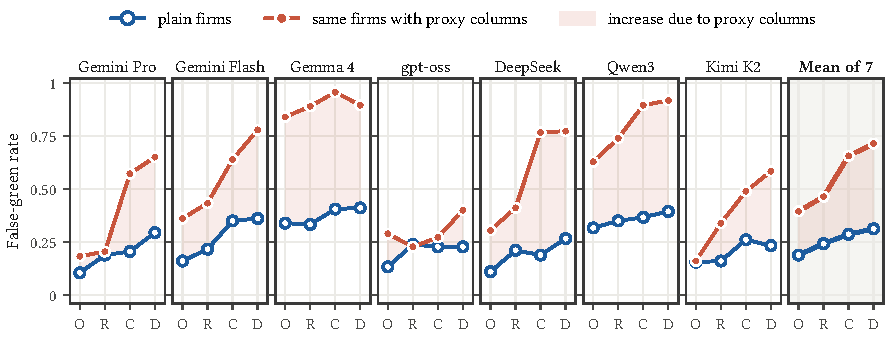
\includegraphics[width=\textwidth]{figures/fig_study3_multiples.pdf}
\caption{False-green rate on the 180 unassessable pairs of the Study 3 firms under the four schemas (O offered, R removed-only, C closed, D dashboard), for plain firms and the same firms with proxy columns. Shading marks where proxy columns raise the rate. Rates are per cell; the tests in Table 3 are paired.}\label{fig:fig_study3_multiples}
\end{figure*}

\begin{table*}[t]
\centering\footnotesize\setlength{\tabcolsep}{4pt}
\caption{The four declared tests of Study 3, with robustness checks.}
\label{tab:3}
\begin{adjustbox}{max width=\textwidth}
\begin{tabular}{lrlrrr}
\toprule
\textbf{Test} & \textbf{Effect [95\% CI]} & \textbf{Exact p (Holm)} & \textbf{Firm-weighted effect, exact p} & \textbf{Drop one model} & \textbf{Drop one firm} \\
\midrule
P1 Abstention (proxy firms) & +0.259 [+0.20, +0.33] & <0.001 & +0.203 (p < 0.001) & +0.226 to +0.306 & +0.227 to +0.271 \\
P2 Definition and warning (proxy firms) & +0.084 [+0.04, +0.12] & 0.001 & +0.051 (p = 0.028) & +0.067 to +0.099 & +0.065 to +0.091 \\
P3 Proxy columns, dashboard & +0.427 [+0.29, +0.56] & <0.001 & +0.244 (p = 0.021) & +0.407 to +0.469 & +0.353 to +0.449 \\
P4 Proxy columns, offered & +0.217 [+0.15, +0.29] & <0.001 & +0.237 (p = 0.002) & +0.170 to +0.244 & +0.200 to +0.230 \\
\bottomrule
\end{tabular}
\end{adjustbox}
\par\vspace{3pt}\begin{minipage}{\textwidth}\scriptsize Effect: change in false-green rate, pooled over seven models with equal weight, paired on unassessable pairs answered in both cells; interval from the declared bootstrap over 18 firm-by-rule clusters. Exact p: sign-flip permutation over those 18 clusters (all 262,144 patterns), Holm across the four tests. Firm-weighted: each of the 12 firms weighted equally, exact sign-flip over firms (4,096 patterns). Drop one: range of the pooled effect with any one model, or any one firm, left out. All columns after the first were computed after the results.\end{minipage}
\end{table*}

\subsection{Design}\label{sec:6.1}
Study 3 was declared in a file committed before any call (commit \texttt{\path|e1baaeb|}), with its analysis script: twelve fresh generated firms (504 pairs, 180 unassessable), each rendered plain and with proxy columns, under the four schemas, with seven models from five developers, once per cell; every cell answered at least 456 of 504 pairs. Contrasts are paired on pairs answered in both cells and averaged over models with equal weight. The declared inference is a bootstrap over the 18 (firm, rule) clusters of unassessable pairs. Four hypotheses predicted increases: \textbf{P1} the abstention effect and \textbf{P2} the definition-and-warning effect, on proxy-column firms; \textbf{P3} and \textbf{P4} the proxy-column effect under the dashboard and offered schemas.

\begin{figure*}[t]\centering
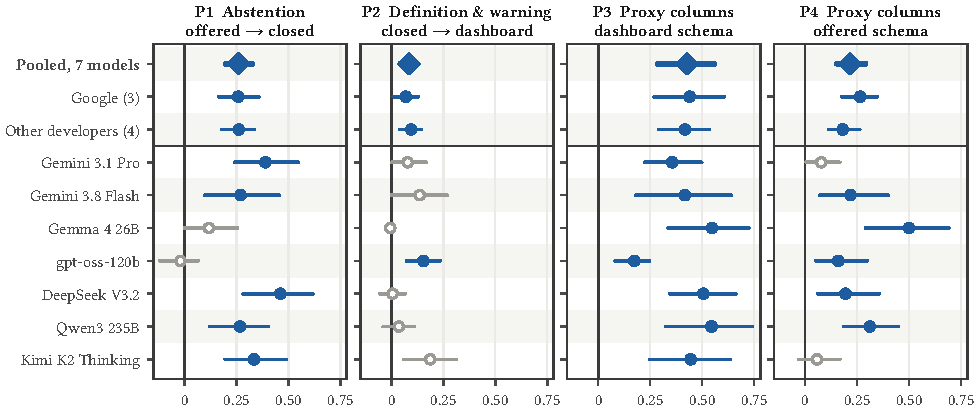
\includegraphics[width=\textwidth]{figures/fig_forest.pdf}
\caption{The declared tests per model and by developer group, with 95\% bootstrap intervals. Filled markers are significant after Holm correction within their family; hollow grey markers are not. Pooled effects are robust; per-model effects vary, most of all P2.}\label{fig:fig_forest}
\end{figure*}

\begin{figure*}[t]\centering
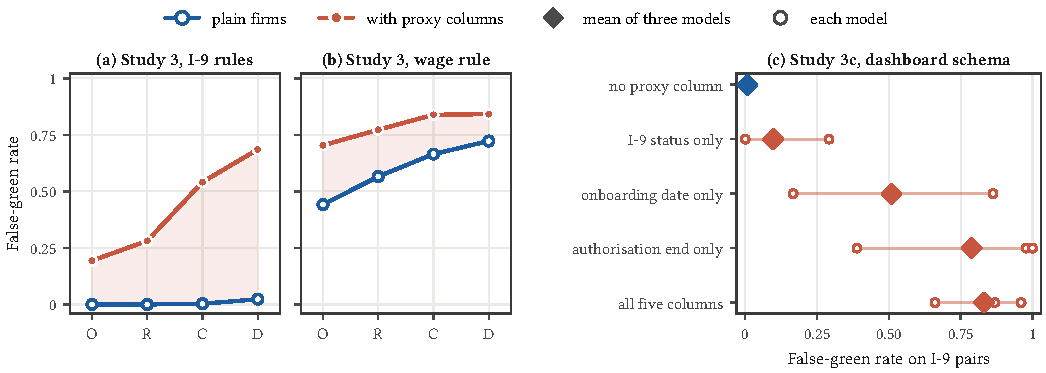
\includegraphics[width=\textwidth]{figures/fig_i9.pdf}
\caption{Where proxy columns act. (a, b) Study 3 false-green rates by rule family under the four schemas (I-9 pairs from 3 firms, wage pairs from 9). (c) Study 3c, ten further firms that withhold the I-9 export, dashboard schema: with no proxy column, with each I-9 proxy column alone (scored on the pairs it bears on) and with all five; diamonds are the mean of three models, circles the models.}\label{fig:fig_i9}
\end{figure*}

\subsection{Results}\label{sec:6.2}
All four were confirmed (Table 3, Figure 2). The bootstrap p-values all sit at its floor (0.002 after correction), so we add an exact sign-flip permutation test, which gives Holm-adjusted p ≤ 0.0013 for all four. Two features of the design temper the headline numbers. The 18 clusters are unbalanced: the I-9 pairs (99) come from only three firms that withhold the I-9 export, and the wage pairs (81) from nine. Weighting the twelve firms equally instead of the pairs, every effect stays positive and significant (exact p from < 0.001 to 0.028), but P3 falls to +0.244, because the large I-9 effect then counts for three firms rather than 99 pairs. Rules within a firm share its records and its withholding draw, so the cluster test treats them as exchangeable where the firm test does not; we read the firm-weighted values as the conservative magnitudes and the pooled ones as specific to this mix of firms. Dropping any one model or any one firm leaves every effect positive.

False greens are not the only wrong answer on an unassessable pair. Averaged over the seven models, on proxy-column firms with abstention offered, 0.517 of unassessable pairs were answered \texttt{\path|needs_evidence|}, 0.395 \texttt{\path|pass|} and 0.045 \texttt{\path|fail|}; under the dashboard schema, where no correct answer exists, 0.713 were \texttt{\path|pass|} and 0.237 \texttt{\path|fail|} (Appendix Figure 9).

The models differ (Figure 3). The proxy-column effect under the dashboard schema is significant for all seven, and under the offered schema for five (not Gemini 3.1 Pro or Kimi K2). The abstention effect is significant for five (not Gemma 4 or gpt-oss-120b), the definition-and-warning effect for one (gpt-oss-120b). Removing only \texttt{\path|needs_evidence|} raised false greens by 0.080 pooled (p = 0.004). The declared interaction, a larger definition-and-warning effect on proxy-column firms, was not found (+0.048 [−0.01, 0.10], p = 0.10). On plain firms both schema effects are present but smaller (exploratory: +0.093 and +0.035).

\begin{table*}[t]
\centering\footnotesize\setlength{\tabcolsep}{4pt}
\caption{The column cited as evidence on each false green, proxy-column firms.}
\label{tab:4}
\begin{adjustbox}{max width=\textwidth}
\begin{tabular}{llrrrr}
\toprule
\textbf{Rule family} & \textbf{Schema} & \textbf{False greens} & \textbf{Citing a planted proxy column} & \textbf{Per model} & \textbf{Citing the LCA offered wage} \\
\midrule
I-9 (three rules) & offered & 134 & 118 (88\%) & 50\%–100\% & 0 (0\%) \\
I-9 (three rules) & dashboard & 462 & 276 (60\%) & 0\%–100\% & 0 (0\%) \\
LCA required wage & offered & 364 & 123 (34\%) & 4\%–77\% & 119 (33\%) \\
LCA required wage & dashboard & 437 & 124 (28\%) & 0\%–71\% & 45 (10\%) \\
\bottomrule
\end{tabular}
\end{adjustbox}
\par\vspace{3pt}\begin{minipage}{\textwidth}\scriptsize Study 3 proxy-column firms, pooled over the seven models; per model: range of the share citing a planted column among models with at least five false greens. The column is the evidence field the reply line names, a self-report. The I-9 status column was never cited. Exploratory.\end{minipage}
\end{table*}

\subsection{Two declared follow-ups}\label{sec:6.3}
\textbf{Study 3b: a reworded prompt.} Each condition had been tested in one wording. We reworded every instruction sentence of the offered and dashboard prompts, keeping meaning and verdict tokens, and re-ran the Study 3 firms with the three Google models (declared before any call; the four other developers' models were not re-run, because their cloud billing had not yet posted). All three declared tests replicated (Holm-adjusted p = 0.0015 each, the bootstrap's floor). Proxy columns raised the false-green rate by 0.483 under the reworded dashboard schema and by 0.301 under the reworded offered schema, against 0.440 and 0.265 for the same three models in the original wording; moving from the offered to the dashboard schema on proxy-column firms raised it by 0.340, against 0.321.

\textbf{Study 3c: more I-9 firms, one column at a time.} To test the I-9 effect on more than three firms, and to ask which column carries it, we drew ten fresh firms that all withhold the I-9 export and rendered each plain, with all five proxy columns, and with each I-9 proxy column alone, with the same three models (declared before any call; firm-level exact permutation tests; Figure 4). In Study 3 the I-9 effect rested on three firms: models called 0.000 to 0.023 of plain-firm I-9 pairs compliant across the four schemas, and 0.193 under the offered and 0.686 under the dashboard schema once proxy columns were present (the wage rule, whose plain firms already show the LCA's offered wage, drew false greens on 0.442 of pairs even there with abstention offered). On the ten new firms all five declared tests were confirmed (exact p ≤ 0.004, Holm-adjusted ≤ 0.010, positive in at least nine firms). All five columns together raised the I-9 false-green rate by 0.822 under the dashboard schema and by 0.302 under the offered schema. One column at a time, the onboarding date raised it by 0.509 on Section 1 and 2 pairs and the current authorisation's end date by 0.759 on reverification pairs, while the I-9 status flag raised it by only 0.097, almost entirely through Gemma 4. Models take a date or an amount that looks like the required one as evidence far more readily than a status flag. The reverification case is the most defensible proxy: a current authorisation implies, without showing, a timely reverification.

\subsection{Study 4: what the effects are made of}\label{sec:6.4}
Study 4, declared before any call (commit \texttt{\path|0c874fc|}), reuses the ten Study 3c firms and the three Google models to take both effects apart (Table 5, Figure 5). Contrasts are paired on pairs answered in both cells, a conditional estimand; cell rates are over answered pairs, and coverage is in Appendix C.9.

\textbf{Names and values.} Under the offered schema, the proxy values under neutral column names (\texttt{\path|rosterField1|}–\texttt{\path|5|}) raised false greens by only 0.052 over plain firms, and five irrelevant columns of the same types and positions by 0.004. The named proxy columns raised them 0.249 more than their renamed twins (H1) and 0.298 more than irrelevant columns (H2). Under the dashboard schema, where every pair must be decided, the renamed values alone added 0.668. For these models, names matter when a model may abstain, and when it must decide plausible values suffice; two other developers' models do not need the names (§6.7). Gemma 4 accounts for 82\% of the named-versus-renamed difference in false-green counts, so H1 rests mostly on one model.

\textbf{One direction.} Proxy columns whose values suggest a breach (an I-9 status of ``Incomplete'', onboarding ten or more days after hire, an authorisation that has ended) moved few answers to \texttt{\path|fail|}: +0.025 (H3, Holm p = 0.047), all from Gemma 4. Gemini 3.1 Pro and 3.8 Flash answered \texttt{\path|needs_evidence|} on all 330 such pairs, although they took favourable proxies as evidence of compliance; Gemma 4 answered \texttt{\path|pass|} on 89 of them, accepting the column's presence whatever it said. The proxy effect is therefore not symmetric evidence substitution: reassuring proxies are accepted and damning ones discounted, which is the direction a false green needs.

\textbf{Menu parts.} In a 2×2×2 factorial of the verdict menu on proxy-column firms, removing the two abstaining verdicts raised false greens by 0.384 (H4) and removing the warning by 0.093 (H6). Replacing the evidence-anchored definitions of \texttt{\path|pass|} and \texttt{\path|fail|} with bare ones changed them by −0.039 (H5, Holm p = 0.080, not confirmed), if anything downward. The parts interact (exploratory; the declaration listed interactions as descriptive): the warning mattered only without the abstaining verdicts (+0.179, against +0.007 with them), and without them bare definitions \emph{lowered} false greens (−0.093). Study 3's definition-and-warning effect (P2) is therefore more plausibly the warning's than the definitions', although Study 4's menus are worded differently. On plain firms no part moved false greens by more than 0.019.

\textbf{An evidence-first prompt.} Adding to the offered menu a requirement to name, as \texttt{\path|<export>.<column>|}, the column that is itself the required record, with two examples and a restated rule to abstain when it is absent, lowered false greens on proxy-column firms from 0.302 to 0.228 (H7, Holm p = 0.047). The change is a bundle, and the reply format still puts the verdict before the evidence field, so it does not isolate ordering. It lowered false greens for all three models: Gemini 3.1 Pro to zero, Flash from 0.115 to 0.049, and Gemma 4 from 0.770 to 0.636, the largest drop but still the highest rate; none of Gemma 4's 210 remaining \texttt{\path|pass|} answers named the I-9 export. No model's recall over all violations fell, but on plain firms Gemma 4 left 3 of 30 violations and 9 of 60 controls unanswered under it. A deterministic gate that routes a rule to \texttt{\path|needs_evidence|} when an export it needs is absent removes every false green here, but it reads the same rule-to-export mapping the generator uses to withhold evidence, so the result is guaranteed by construction: a structural baseline, not evidence for a safeguard against partial, stale or conflicting records.

\textbf{Repeat runs.} Running the original plain and proxy cells twice more (not the factorial, the controls or the evidence-first prompt) moved per-model false-green rates by at most 0.100, and the proxy effect stayed between 0.300 and 0.347 under the offered schema and between 0.798 and 0.822 under the dashboard schema.

\begin{table*}[t]
\centering\footnotesize\setlength{\tabcolsep}{4pt}
\caption{The seven declared tests of Study 4.}
\label{tab:5}
\begin{adjustbox}{max width=\textwidth}
\begin{tabular}{llrrr}
\toprule
\textbf{Test} & \textbf{Contrast} & \textbf{Effect [95\% CI]} & \textbf{Firms + / −} & \textbf{Exact p (Holm)} \\
\midrule
H1 Names & proxy columns − same values, neutral names & +0.249 [+0.21, +0.29] & 10 / 0 & 0.014 \\
H2 Meaning & proxy columns − irrelevant columns & +0.298 [+0.27, +0.33] & 10 / 0 & 0.014 \\
H3 Direction & adverse proxies − none; outcome \texttt{fail} & +0.025 [+0.01, +0.04] & 7 / 0 & 0.047 \\
H4 Abstaining verdicts & removed − listed (factorial) & +0.384 [+0.37, +0.40] & 10 / 0 & 0.014 \\
H5 Definitions & bare − evidence-anchored (factorial) & -0.039 [-0.08, -0.00] & 3 / 7 & 0.080 \\
H6 Warning & absent − present (factorial) & +0.093 [+0.07, +0.12] & 10 / 0 & 0.014 \\
H7 Evidence-first prompt & offered − offered with evidence-first prompt & +0.074 [+0.03, +0.13] & 7 / 1 & 0.047 \\
\bottomrule
\end{tabular}
\end{adjustbox}
\par\vspace{3pt}\begin{minipage}{\textwidth}\scriptsize Ten Study 3c firms (330 unassessable I-9 pairs), three Google models. Outcome: false green (\texttt{pass} on an unassessable pair) except H3 (\texttt{fail}). H1-H3 and H7 use the offered schema; H4-H6 average the four factorial menus on each side of the switch. All tests except H3 are on proxy-column firms. Paired, averaged within firm and model then over models; interval from a firm bootstrap; exact sign-flip over the ten firms (1,024 patterns), Holm across the seven tests. Declared before any call.\end{minipage}
\end{table*}

\begin{figure*}[t]\centering
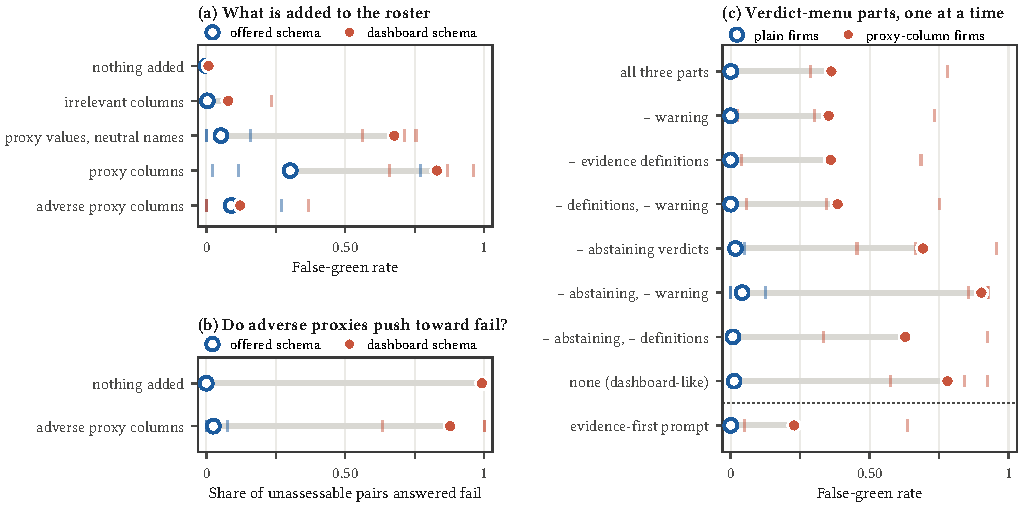
\includegraphics[width=\textwidth]{figures/fig_study4.pdf}
\caption{Study 4: ten firms that withhold the I-9 export, three models; dots are means over models, ticks individual models. (a) False-green rate by what is added to the roster, under the offered and dashboard schemas. (b) Share of unassessable pairs answered fail with nothing added and with proxies that suggest a breach. (c) The verdict menu with its three parts (abstaining verdicts, evidence-anchored definitions, warning) removed one or more at a time, and the offered menu with the evidence-first prompt, on plain and proxy-column firms.}\label{fig:fig_study4}
\end{figure*}

\subsection{Study 5: real LCA records}\label{sec:6.5}
Study 5, declared before any call (commit \texttt{\path|bc4a796|}), replaces generated LCAs with 120 certified H-1B LCAs drawn by a fixed rule from the Department of Labor's public FY2026 Q3 disclosure file (Appendix A). A disclosure states the offered and prevailing wages but never the wages paid, so whether the required wage was paid (20 C.F.R. 655.731) cannot be decided from it; the label needs no legal interpretation. The rows form 12 firms of 10, and each worker sits on a roster whose columns follow BambooHR's export format, with or without its \texttt{\path|Pay Rate|} field, a salary of record set to the LCA's offered wage. A third arm adds a payroll register and an actual-wage export, making every pair decidable.

With abstention offered and no pay field, Gemini 3.1 Pro and 3.8 Flash answered \texttt{\path|needs_evidence|} on every pair they answered (Flash answered 119 of 120), while Gemma 4 called 0.825 of them compliant. Adding the roster's pay fields raised false greens by 0.236 (R1, Holm p = 0.016; paired on pairs answered in both arms, so the firm where Gemma 4 answered no salary-arm pair averages the other two models; the equally weighted all-pair rates are 0.275 and 0.469): Flash then called half the pairs compliant and cited \texttt{\path|Pay Rate|} on 40 of its 60, while Pro stayed at zero. Under the dashboard schema false greens were 0.861 without the pay field and rose a further 0.108 with it (R2, not confirmed); removing the abstaining verdicts raised them by 0.586 (R3, Holm p = 0.0015). Given the payroll register, Pro and Flash detected every underpaid worker with no false alarm, so their abstention was not indiscriminate; Gemma 4 detected 0.066 of them. With real LCA records inside constructed employers, the wage rule thus shows both effects of Study 3, the proxy effect with abstention offered in two of three models.

\subsection{What models rely on}\label{sec:6.6}
Every reply line names the evidence field relied on. This is the model's own report, and stated reasons need not be the cause (Turpin et al., 2023); the causal evidence is the paired contrasts of Studies 3, 3c and 4, and the citations only show what models say they used (Table 4). On proxy-column firms, 1,376 of the 2,807 false greens (49\%) cite one of the five planted columns, and for the I-9 rules under the offered schema 118 of 134 (88\%), almost all the onboarding date or the current authorisation's end date. On plain firms, wage-rule false greens most often cite the LCA's offered wage. Under the dashboard schema more false greens cite other fields, consistent with a schema that asks only whether the obligation is satisfied.

Detection does not bring safety. On the proxy-column firms, Gemini 3.1 Pro, Gemini 3.8 Flash, gpt-oss-120b and Kimi K2 detect at least 0.920 of violations with abstention offered, yet call 0.161 to 0.361 of unassessable pairs compliant. Across the seven models recall and false-green rate are negatively related, so higher recall helps, but none of the high-recall models comes near zero (Appendix Figure 10). Proxy columns change the false-alarm rate on conforming controls by at most 0.038 with abstention offered and 0.080 under any schema, so their cost falls mostly on the false-green side.

\subsection{Study 6: two more developers}\label{sec:6.7}
Studies 3b–5 used only Google's models. Study 6, declared before any call (commit \texttt{\path|d03c7ee|}), ran every declared Study 4 and Study 5 cell, unchanged, on DeepSeek V3.2 and GLM-5.2 (Zhipu AI), current models from other developers that Google serves on Vertex as pay-per-token models. Averaged over the two models, as declared, seven of the ten tests replicated with the same sign (Table 6):

\begin{itemize}
\item proxy columns raised false greens more than irrelevant columns did (+0.118);
\item removing the abstaining verdicts raised them (+0.645);
\item the evidence-first prompt lowered them (−0.097);
\item on the real LCA records, the pay fields raised them by 0.562 with abstention offered, and removing abstention raised them by 0.892.
\end{itemize}

Averages can hide disagreement between models (Table 19 gives every model's effect):

\begin{itemize}
\item \textbf{Warning (H6).} The warning's effect came from DeepSeek (+0.059); for GLM-5.2 it was −0.005.
\item \textbf{Names (H1).} The pooled names advantage did not replicate (−0.009) because the two models went opposite ways. Named proxies raised DeepSeek's false greens by 0.091 over renamed ones and lowered GLM-5.2's by 0.091; GLM-5.2 called 0.211 of unassessable pairs compliant from the renamed values. The pooled null shows that names are not necessary for the effect, not that names and values are equivalent.
\item \textbf{Definitions (H5).} Bare definitions \emph{raised} false greens for both models (+0.056), the reverse of the Google models' non-significant −0.039. So the names and the wording of \texttt{\path|pass|} matter in a model-specific way, while the abstaining verdicts and the proxy columns matter for all five models.
\item \textbf{Breach proxies (H3).} Both models moved some unassessable pairs to \texttt{\path|fail|} when the proxies suggested a breach (+0.064), so their substitution runs in both directions.
\item \textbf{Cost of the evidence-first prompt.} For DeepSeek the prompt cut false greens from 0.121 to 0.015, but it also cut violation recall from 0.133 to 0.067 and raised false alarms on controls from 0.167 to 0.200. It traded one error for others.
\end{itemize}

Given complete records, GLM-5.2 detected every underpaid worker and DeepSeek V3.2 none.

\begin{table*}[t]
\centering\footnotesize\setlength{\tabcolsep}{4pt}
\caption{The declared tests of Studies 4 and 5 on two model sets.}
\label{tab:6}
\begin{adjustbox}{max width=\textwidth}
\begin{tabular}{lrrl}
\toprule
\textbf{Test} & \textbf{Gemini 3.1 Pro, 3.8 Flash, Gemma 4} & \textbf{DeepSeek V3.2, GLM-5.2} & \textbf{Replicated} \\
\midrule
H1 Names (proxy − renamed) & +0.249 (p 0.014) & -0.009 (p 0.828, n.s.) & no \\
H2 Meaning (proxy − irrelevant) & +0.298 (p 0.014) & +0.118 (p 0.014) & yes \\
H3 Direction (adverse, \texttt{fail}) & +0.025 (p 0.047) & +0.064 (p 0.023) & yes \\
H4 Abstaining verdicts removed & +0.384 (p 0.014) & +0.645 (p 0.014) & yes \\
H5 Bare definitions & -0.039 (p 0.080, n.s.) & +0.056 (p 0.014) & no (opposite sign) \\
H6 Warning removed & +0.093 (p 0.014) & +0.028 (p 0.043) & yes \\
H7 Evidence-first prompt & +0.074 (p 0.047) & +0.097 (p 0.014) & yes \\
R1 Salary of record, offered (real LCAs) & +0.236 (p 0.016) & +0.562 (p 0.002) & yes \\
R2 Salary of record, dashboard (real LCAs) & +0.108 (p 0.219, n.s.) & +0.046 (p 0.188, n.s.) & both n.s. \\
R3 Dashboard − offered (real LCAs) & +0.586 (p 0.001) & +0.892 (p 0.001) & yes \\
\bottomrule
\end{tabular}
\end{adjustbox}
\par\vspace{3pt}\begin{minipage}{\textwidth}\scriptsize Effects on the false-green rate (H3: on \texttt{fail}), each model weighted equally; Holm-adjusted exact sign-flip p over firms (ten for H, twelve for R), Holm within each study and model set as declared. Study 6 ran the declared Study 4 and 5 cells unchanged on two more developers' models. Contrasts are paired on pairs answered in both cells; where a model answered none of a firm's pairs in a cell, that firm's contrast averages the remaining models. Per-model effects are in Table 19.\end{minipage}
\end{table*}

\subsection{Study 7: which pay field}\label{sec:6.8}
Study 5's salary arm adds three roster fields at once: \texttt{\path|Pay Rate|}, \texttt{\path|Pay Type|} and \texttt{\path|Pay Schedule|}. Study 7, declared before any call (commit \texttt{\path|75a21a1|}), added each part alone to the twelve real-LCA firms under the offered schema, on all five models.

\begin{itemize}
\item \textbf{\texttt{\path|Pay Rate|} alone} raised false greens by 0.227 (W1, Holm p = 0.001, positive in all twelve firms): +0.775 for DeepSeek V3.2, +0.182 for Gemma 4, +0.160 for Gemini 3.8 Flash, and zero for Gemini 3.1 Pro and GLM-5.2.
\item \textbf{Pay type and schedule alone} added 0.067 (W2, not confirmed).
\item \textbf{The combination.} For two models it went further than the salary alone: relative to \texttt{\path|Pay Rate|} alone, all three fields raised Flash's false greens by 0.342 and GLM-5.2's by 0.244.
\end{itemize}

The salary of record alone induces false greens in three of five models, and the surrounding pay context strengthens the response in some. Study 7's five-model estimate is not a share of Study 5's three-model one: restricted to Study 5's three models, \texttt{\path|Pay Rate|} alone gives +0.108 against +0.236 for the three fields together. GLM-5.2 answered 100 of 120 pairs in the \texttt{\path|Pay Rate|} arm.

\subsection{Study 8: fresh firms, repeat runs and two wage controls}\label{sec:6.9}
Study 6 reused the Study 3c firms and ran once; Study 5's \texttt{\path|Pay Rate|} equalled the LCA's offered wage; and its complete arm made the greater-of rule trivial. Study 8, declared before any call (commit \texttt{\path|ec2a325|}), addressed all three.

\textbf{Fresh firms, repeat runs.} Ten new firms that withhold the I-9 export were rendered plain, with proxy columns, with irrelevant columns and with renamed proxy values. All five models ran them twice under both schemas. All four declared tests were confirmed (Holm p = 0.010 each), positive in all ten firms. The pooled estimates from the two runs agreed to within 0.02, though single models moved more (GLM-5.2's F4 by 0.076):

\begin{table}[t]
\centering\footnotesize\setlength{\tabcolsep}{4pt}
\begin{tabularx}{\columnwidth}{>{\raggedright\arraybackslash}Xl}
\toprule
\textbf{Test} & \textbf{Effect} \\
\midrule
F1: proxy columns over none, offered & +0.224 \\
F2: proxy columns over irrelevant columns & +0.224 \\
F3: dashboard over offered, on proxy firms & +0.608 \\
F4: renamed values over none, dashboard & +0.700 \\
\bottomrule
\end{tabularx}
\end{table}

The proxy effect under the offered schema was positive for every model, from +0.038 (Gemini 3.1 Pro) to +0.795 (Gemma 4). Proxy columns are now tested on 32 firms.

\textbf{Wage controls.} On the real-LCA firms:

\begin{itemize}
\item \textbf{G1.} \texttt{\path|Pay Rate|} set 7\% above the LCA's offered wage still raised false greens by 0.247 (Holm p = 0.006, positive in eleven firms), so the effect does not depend on the roster repeating the LCA's number.
\item \textbf{G2.} A complete arm whose actual-wage export exceeds the offered wage contains underpayments visible only under the greater-of rule. We found no significant pooled difference between recall on these 38 underpayments and on the 24 below the offered wage (G2, −0.028 [−0.115, +0.053], ten firms, not confirmed); this does not show the two are detected equally often. Gemini 3.1 Pro and GLM-5.2 detected every greater-of-only underpayment and Flash 0.947. DeepSeek V3.2 detected 0.526 of them against 0.667 of those below the offered wage, and also flagged 0.569 of correctly paid workers.
\end{itemize}

The lowest coverage in Part A was 291 of 330 pairs (GLM-5.2 again exceeding its output budget on renamed values under the dashboard schema).

\section{The exploratory study that generated the hypotheses}\label{sec:7}
\begin{figure*}[t]\centering
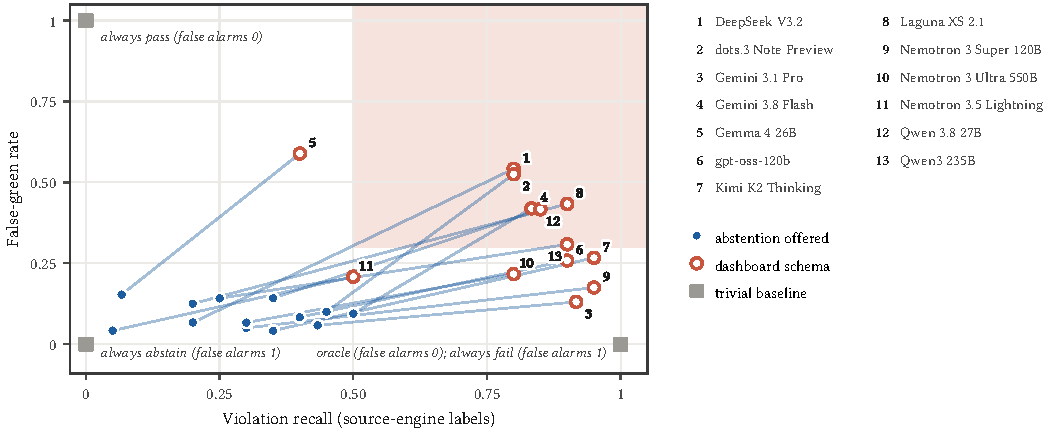
\includegraphics[width=\textwidth]{figures/fig_separation.pdf}
\caption{The anchor subset, exploratory: each model under the offered schema (filled) and the dashboard schema (open), joined by a line; numbers refer to the key. Without the abstention every model moves up and right, buying recall with false greens; the shaded region marks high recall with many false greens. Recall is measured against the source engine's contested violation labels and is shown only for direction. Grey squares are trivial baselines, labelled with their false-alarm rate on conforming pairs, which separates the oracle from always\_fail.}\label{fig:fig_separation}
\end{figure*}

Before Study 3, all thirteen models were run on a declared 140-pair subset of the anchor firm, not all 221 pairs, for the free-tier budget (every planted violation and 120 evidence requests), most once, three Google models three times (their runs differed in false-green rate by at most 0.142).

With abstention offered the thirteen models report 0.042 to 0.153 of unassessable pairs as satisfied, and 0.131 to 0.589 under the dashboard schema (Figure 6); the dashboard schema raised the rate significantly for eight of the nine models tested for it, and the four added later were run descriptively. Decomposing the schema for the three repeated-run models showed that each failed through a different route: Gemma 4 when \texttt{\path|needs_evidence|} alone was removed, Gemini 3.8 Flash when every non-committal verdict was removed, and Gemini 3.1 Pro only when \texttt{\path|pass|} was redefined; Pro otherwise sent unassessable pairs to \texttt{\path|unmonitored|} or \texttt{\path|fail|}. False greens concentrated where a populated column sat beside the missing evidence. Two of the excerpts selected by a rule fixed before any reply was read: Qwen 3.8 27B and dots.3 cited an unitemized payroll deduction total as evidence that no prohibited fee was charged, and Nemotron 3.5 Lightning and Laguna XS 2.1 inferred the physical examination of I-9 documents from the presence of a document title. These observations are what Study 3 tested.

\section{Discussion}\label{sec:8}
The experiments establish risks more firmly than remedies. Two parts of a verdict menu lowered false greens, a verdict for ``could not tell'' and, when that verdict was absent, the warning that a missing record is not a record in order; the wording of \texttt{\path|pass|} mattered for some models and not others; with both in place, false-green rates of 0.04 to 0.15 remain on the anchor firm and 0.16 to 0.84 on proxy-column firms. Export columns whose names resemble required evidence are a hazard that no menu removed, and for Google's models the bias they create runs toward green. An evidence-first prompt lowered false greens for all five models, but left Gemma 4 at 0.636 and cost DeepSeek V3.2 half its violation recall, which suggests checking outside the model that the required record exists before asking for a verdict; our generator cannot test such a check, because its gaps are whole exports. We have not compared such safeguards with human reviewers or on real employer data. That models respond to wording is well known (Sclar et al., 2024); the effects here survive a rewording, replicate on fresh firms, on repeat runs, on real LCA records and on two other developers' models, and the proxy effect involves no change to the prompt. Whether a proxy-based \texttt{\path|pass|} is an error depends on the standard (§3): it is a reasonable triage guess, and a claim made without the record under the standard a monitoring product implies.

\section{Limitations}\label{sec:9}
\begin{itemize}
\item \textbf{No human expert labels or baseline.} No attorney validated any label; the generated labels are re-derived by an AI-written checker sharing the generator's standard, and the anchor labels are qualified by two AI audits. A blind expert workbook is released; only two AI pilot runs have completed it (Appendix I).
\item \textbf{A narrow, synthetic generator.} Four of the rulebook's rules, whole-export withholding, five proxy columns chosen by us, and no generated pair whose answer is \texttt{\path|unmonitored|}; no partial records, scanned documents or OCR. Study 4's controls cover the I-9 rules only; Study 5's LCAs are real but its rosters and payroll are constructed, and it covers the wage rule only. Two rules simplify the law (a timely extension can allow 240 more days before reverification; ``business day'' is not defined in the handbook).
\item \textbf{Statistics.} Study 3 has 18 clusters, its I-9 effect three firms (Studies 3c and 4 add ten), and pooled estimates weight particular models equally and depend on the mix of firms. Study 3's cells were run once; repeat runs in Study 4 moved per-model rates by at most 0.100, and Study 8's pooled estimates from two runs on fresh firms agreed to within 0.02 (single models by up to 0.076).
\item \textbf{Model coverage is narrow.} No closed OpenAI, Anthropic or xAI model was evaluated: on Vertex AI they are sold through Google Cloud Marketplace, which the study's cloud credits do not cover, and the study used no other funds; Studies 3b and 3c use only the three Google models, and Studies 4 and 5 add two other developers' open models (Study 6); several endpoints are previews that will be retired.
\item \textbf{One domain.} We conjecture, and do not show, that the failure generalises.
\end{itemize}

\section*{Ethics, competing interests and AI use}
Every employer record is synthetic except Study 5's LCAs, which are public DOL disclosures used without employer names. A high score does not show a system fit for use, and the labels are not a training set. The author works for Settle AI Inc., which builds commercial compliance software; the anchor labels and the rulebook derive from its engine, which is not evaluated, and the audits that weaken those labels are reported in full. No model provider was consulted. Anthropic's Claude wrote the code, ran the experiments and drafted the text; separate agents performed the first label audit and wrote the reference checker, and Gemini 3.1 Pro performed the second audit, all reported as AI checks. Every number is recomputed from released artifacts by \texttt{\path|scripts/verify_paper.py|}; the author is responsible for the content. Code is released under Apache-2.0 and data under CC-BY-4.0.

\FloatBarrier
\section*{References}\label{sec:refs}
\begingroup\small\raggedright\setlength{\parindent}{-1.2em}\setlength{\leftskip}{1.2em}\setlength{\parskip}{2pt}
Afsharrad, A. and Mousavi, S. S. (2026). ImmigrationReason: A Structured Dataset of U.S. Immigration Appeals for Legal Reasoning Research. arXiv preprint arXiv:2608.20391. \url{https://arxiv.org/abs/2608.20391}

Aly, R., Guo, Z., Schlichtkrull, M., Thorne, J., Vlachos, A., Christodoulopoulos, C., Cocarascu, O. and Mittal, A. (2021). FEVEROUS: Fact Extraction and VERification Over Unstructured and Structured information. NeurIPS 2021 Datasets and Benchmarks Track. \url{https://arxiv.org/abs/2106.05707}

Amaral, O., Abualhaija, S., Torre, D., Sabetzadeh, M. and Briand, L. C. (2022). AI-enabled Automation for Completeness Checking of Privacy Policies. IEEE Transactions on Software Engineering 48(11). \url{https://doi.org/10.1109/TSE.2021.3124332}

Chalkidis, I., Jana, A., Hartung, D., Bommarito, M., Androutsopoulos, I., Katz, D. M. and Aletras, N. (2022). LexGLUE: A Benchmark Dataset for Legal Language Understanding in English. Proceedings of ACL 2022. \url{https://aclanthology.org/2022.acl-long.297}

Chow, C. (1970). On optimum recognition error and reject tradeoff. IEEE Transactions on Information Theory 16(1):41-46. \url{https://doi.org/10.1109/TIT.1970.1054406}

Dahl, M., Magesh, V., Suzgun, M. and Ho, D. E. (2024). Large Legal Fictions: Profiling Legal Hallucinations in Large Language Models. Journal of Legal Analysis 16(1):64-93. \url{https://arxiv.org/abs/2401.01301}

Dou, G., Brena, L., Deo, A., Jurayj, W., Zhang, J., Holzenberger, N. and Van Durme, B. (2026). DeonticBench: A Benchmark for Reasoning over Rules. arXiv preprint arXiv:2604.04443. \url{https://arxiv.org/abs/2604.04443}

El-Yaniv, R. and Wiener, Y. (2010). On the Foundations of Noise-free Selective Classification. Journal of Machine Learning Research 11:1605-1641. \url{https://jmlr.org/papers/v11/el-yaniv10a.html}

Fei, Z., Shen, X., Zhu, D., Zhou, F., Han, Z., Zhang, S., Chen, K., Shen, Z. and Ge, J. (2024). LawBench: Benchmarking Legal Knowledge of Large Language Models. Proceedings of EMNLP 2024. \url{https://aclanthology.org/2024.emnlp-main.452}

Fu, Y., Kang, Y. and Zhao, Y. (2026). CalBrief: A Pilot Diagnostic Benchmark for Evidence-Calibrated Scientific Briefing with Large Language Models. arXiv preprint arXiv:2606.27383. \url{https://arxiv.org/abs/2606.27383}

Geifman, Y. and El-Yaniv, R. (2017). Selective Classification for Deep Neural Networks. Advances in Neural Information Processing Systems 30. \url{https://arxiv.org/abs/1705.08500}

Geirhos, R., Jacobsen, J.-H., Michaelis, C., Zemel, R., Brendel, W., Bethge, M. and Wichmann, F. A. (2020). Shortcut Learning in Deep Neural Networks. Nature Machine Intelligence 2:665-673. \url{https://doi.org/10.1038/s42256-020-00257-z}

Guha, N., Nyarko, J., Ho, D. E., Ré, C., et al. (2023). LegalBench: A Collaboratively Built Benchmark for Measuring Legal Reasoning in Large Language Models. NeurIPS 2023 Datasets and Benchmarks Track. \url{https://arxiv.org/abs/2308.11462}

Guldimann, P., Spiridonov, A., Staab, R., Jovanović, N., Vero, M., Vechev, V., Gueorguieva, A.-M., Balunović, M., Konstantinov, N., Bielik, P., Tsankov, P. and Vechev, M. (2024). COMPL-AI Framework: A Technical Interpretation and LLM Benchmarking Suite for the EU Artificial Intelligence Act. arXiv preprint arXiv:2410.07959. \url{https://arxiv.org/abs/2410.07959}

Guo, K. H., Yan, C., Baidya, A., Brown, K., Gao, X., Xiong, J., Yin, Z. and Malin, B. A. (2026). CLEAR: Revealing How Noise and Ambiguity Degrade Reliability in LLMs for Medicine. arXiv preprint arXiv:2605.01011. \url{https://arxiv.org/abs/2605.01011}

Hendrycks, D., Burns, C., Chen, A. and Ball, S. (2021). CUAD: An Expert-Annotated NLP Dataset for Legal Contract Review. NeurIPS 2021 Datasets and Benchmarks Track. \url{https://arxiv.org/abs/2103.06268}

Joren, H., Zhang, J., Ferng, C.-S., Juan, D.-C., Taly, A. and Rashtchian, C. (2024). Sufficient Context: A New Lens on Retrieval Augmented Generation Systems. arXiv preprint arXiv:2411.06037. \url{https://arxiv.org/abs/2411.06037}

Kadavath, S., Conerly, T., Askell, A., Henighan, T., Drain, D., Perez, E., et al. (2022). Language Models (Mostly) Know What They Know. arXiv preprint arXiv:2207.05221. \url{https://arxiv.org/abs/2207.05221}

Kalai, A. T., Nachum, O., Vempala, S. S. and Zhang, E. (2025). Why Language Models Hallucinate. arXiv preprint arXiv:2509.04664. \url{https://arxiv.org/abs/2509.04664}

Kirichenko, P., Ibrahim, M., Chaudhuri, K. and Bell, S. J. (2025). AbstentionBench: Reasoning LLMs Fail on Unanswerable Questions. arXiv preprint arXiv:2506.09038. \url{https://arxiv.org/abs/2506.09038}

Koreeda, Y. and Manning, C. D. (2021). ContractNLI: A Dataset for Document-level Natural Language Inference for Contracts. Findings of EMNLP 2021. \url{https://aclanthology.org/2021.findings-emnlp.164}

Lee, G., Chay, W., Cho, S. and Choi, E. (2024). TrustSQL: Benchmarking Text-to-SQL Reliability with Penalty-Based Scoring. arXiv preprint arXiv:2403.15879. \url{https://arxiv.org/abs/2403.15879}

Lee, G., Hwang, H., Bae, S., Kwon, Y., Shin, W., Yang, S., Seo, M., Kim, J.-Y. and Choi, E. (2022). EHRSQL: A Practical Text-to-SQL Benchmark for Electronic Health Records. NeurIPS 2022 Datasets and Benchmarks Track. \url{https://arxiv.org/abs/2301.07695}

Luo, Y., Jiang, Y., Xie, Q., Lan, L., Cong, L. W., Rao, A. and Song, Y. (2026). ReguSim: Evaluating LLM Agent Rule Grounding in Financial Compliance. arXiv preprint arXiv:2608.19974. \url{https://arxiv.org/abs/2608.19974}

Madhusudhan, N., Madhusudhan, S. T., Yadav, V. and Hashemi, M. (2025). Do LLMs Know When to NOT Answer? Investigating Abstention Abilities of Large Language Models. Proceedings of COLING 2025. \url{https://aclanthology.org/2025.coling-main.627}

Magesh, V., Surani, F., Dahl, M., Suzgun, M., Manning, C. D. and Ho, D. E. (2025). Hallucination-Free? Assessing the Reliability of Leading AI Legal Research Tools. Journal of Empirical Legal Studies 22(2). \url{https://doi.org/10.1111/jels.12413}

Marino, B., Hunter, R., Schnabl, C., Jamali, Z., Kalpakos, M. E., Kashyap, M., Hinton, I., Hanson, A., Nazir, M., Steffek, F., Wen, H. and Lane, N. D. (2025). AIReg-Bench: Benchmarking Language Models That Assess AI Regulation Compliance. arXiv preprint arXiv:2510.01474. \url{https://arxiv.org/abs/2510.01474}

Rajpurkar, P., Jia, R. and Liang, P. (2018). Know What You Don't Know: Unanswerable Questions for SQuAD. Proceedings of ACL 2018. \url{https://aclanthology.org/P18-2124}

Ravichander, A., Black, A. W., Wilson, S., Norton, T. and Sadeh, N. (2019). Question Answering for Privacy Policies: Combining Computational and Legal Perspectives. Proceedings of EMNLP-IJCNLP 2019. \url{https://aclanthology.org/D19-1500}

Röttger, P., Hofmann, V., Pyatkin, V., Hinck, M., Kirk, H. R., Schütze, H. and Hovy, D. (2024). Political Compass or Spinning Arrow? Towards More Meaningful Evaluations for Values and Opinions in Large Language Models. Proceedings of ACL 2024. \url{https://aclanthology.org/2024.acl-long.816}

Sarkar, D. (2026). A Four-Axis Trustworthiness Benchmark for LLM-as-Judge in Principle-Based Regulation. KDD 2026 Workshop on Secure and Trustworthy Large Language Models. arXiv:2608.14329. \url{https://arxiv.org/abs/2608.14329}

Sclar, M., Choi, Y., Tsvetkov, Y. and Suhr, A. (2024). Quantifying Language Models' Sensitivity to Spurious Features in Prompt Design or: How I learned to start worrying about prompt formatting. ICLR 2024. \url{https://arxiv.org/abs/2310.11324}

Shi, F., Chen, X., Misra, K., Scales, N., Dohan, D., Chi, E., Schärli, N. and Zhou, D. (2023). Large Language Models Can Be Easily Distracted by Irrelevant Context. ICML 2023. \url{https://arxiv.org/abs/2302.00093}

Shportun, N. (2026). ImmigrationQA: A Source-Grounded Dataset and Small-Model Adaptation for U.S. Immigration Law. arXiv preprint arXiv:2605.30589. \url{https://arxiv.org/abs/2605.30589}

Solozobov, O. (2026). DEMM-Bench: A Cross-Regime Benchmark for Agent-Runtime Governance-Evidence Sufficiency. arXiv preprint arXiv:2606.20634. \url{https://arxiv.org/abs/2606.20634}

Tallam, K. (2026). Partial Evidence Bench: Benchmarking Authorization-Limited Evidence in Agentic Systems. arXiv preprint arXiv:2605.05379. \url{https://arxiv.org/abs/2605.05379}

Tam, Z. R., Wu, C.-K., Tsai, Y.-L., Lin, C.-Y., Lee, H. and Chen, Y.-N. (2024). Let Me Speak Freely? A Study On The Impact Of Format Restrictions On Large Language Model Performance. Proceedings of EMNLP 2024: Industry Track. \url{https://aclanthology.org/2024.emnlp-industry.91}

Theologitis, M., Dammu, P. P. S., Shah, C. and Suciu, D. (2026). ClaimDB: A Fact Verification Benchmark over Large Structured Data. ACL 2026. arXiv:2601.14698. \url{https://arxiv.org/abs/2601.14698}

Thorne, J., Vlachos, A., Christodoulopoulos, C. and Mittal, A. (2018). FEVER: a Large-scale Dataset for Fact Extraction and VERification. Proceedings of NAACL-HLT 2018. \url{https://aclanthology.org/N18-1074}

Turpin, M., Michael, J., Perez, E. and Bowman, S. R. (2023). Language Models Don't Always Say What They Think: Unfaithful Explanations in Chain-of-Thought Prompting. NeurIPS 2023. \url{https://arxiv.org/abs/2305.04388}

U.S. Department of Labor, Wage and Hour Division (2026). H-1B compliance data by fiscal year. Retrieved 2026-10-07. \url{https://www.dol.gov/agencies/whd/data/charts/h-1b}

U.S. Immigration and Customs Enforcement (2026). Form I-9 Inspection. Fact sheet, retrieved 2026-10-07. \url{https://www.ice.gov/factsheets/i9-inspection}

Wang, B., Gao, Y., Li, Z. and Lou, J.-G. (2023). Know What I don't Know: Handling Ambiguous and Unknown Questions for Text-to-SQL. Findings of ACL 2023. \url{https://aclanthology.org/2023.findings-acl.352}

Wang, J., Wang, M., Zhou, Y., Xing, Z., Liu, Q., Xu, X., Zhang, W. and Zhu, L. (2025). LLM-based HSE Compliance Assessment: Benchmark, Performance, and Advancements. arXiv preprint arXiv:2505.22959. \url{https://arxiv.org/abs/2505.22959}

Wang, N. X. R., Mahajan, D., Danilevsky, M. and Rosenthal, S. (2021). SemEval-2021 Task 9: Fact Verification and Evidence Finding for Tabular Data in Scientific Documents (SEM-TAB-FACTS). Proceedings of SemEval-2021. \url{https://aclanthology.org/2021.semeval-1.39}

Wen, B., Yao, J., Feng, S., Xu, C., Tsvetkov, Y., Howe, B. and Wang, L. L. (2025). Know Your Limits: A Survey of Abstention in Large Language Models. Transactions of the Association for Computational Linguistics. \url{https://aclanthology.org/2025.tacl-1.26}

Yang, Y., Kim, I.-J. and Yoon, D. (2026). PASTA: A Scalable Framework for Multi-Policy AI Compliance Evaluation. Proceedings of CHI 2026. \url{https://doi.org/10.1145/3772318.3790966}

Yin, Z., Sun, Q., Guo, Q., Wu, J., Qiu, X. and Huang, X. (2023). Do Large Language Models Know What They Don't Know? Findings of ACL 2023. \url{https://aclanthology.org/2023.findings-acl.551}

Zhang, J. and El-Gohary, N. M. (2016). Semantic NLP-Based Information Extraction from Construction Regulatory Documents for Automated Compliance Checking. Journal of Computing in Civil Engineering 30(2). \url{https://doi.org/10.1061/(ASCE})CP.1943-5487.0000346

Zheng, L., Guha, N., Anderson, B. R., Henderson, P. and Ho, D. E. (2021). When Does Pretraining Help? Assessing Self-Supervised Learning for Law and the CaseHOLD Dataset. ICAIL 2021. \url{https://arxiv.org/abs/2104.08671}

Zhou, R., Hua, W., Pan, L., Cheng, S., Wu, X., Yu, E. and Wang, W. Y. (2025). RuleArena: A Benchmark for Rule-Guided Reasoning with LLMs in Real-World Scenarios. Proceedings of ACL 2025. \url{https://aclanthology.org/2025.acl-long.27}

---

\endgroup

\clearpage
\onecolumn
\appendix
\section{Reproduction}\label{app:A}
\begin{Verbatim}[breaklines,breakanywhere,fontsize=\scriptsize,frame=single,framerule=0.3pt,rulecolor=\color{fggray}]
python3 tests/test_benchmark.py; python3 tests/test_llm_harness.py; python3 tests/test_freetier.py
python3 scripts/sweep.py --firms 30            # Table 7 (trivial baselines)
python3 scripts/score_views.py                  # anchor study, label views, Table 12
python3 scripts/score_studies.py                # repeated-run study and Study 2
python3 scripts/score_study3.py                 # Study 3, the declared analysis
python3 scripts/study3_exploratory.py           # Section 6.6 (exploratory)
python3 scripts/study3_robustness.py            # Table 3 robustness columns
python3 scripts/score_paraphrase.py             # Study 3b
python3 scripts/score_study3c.py                # Study 3c
python3 scripts/score_study4.py                 # Study 4
python3 scripts/score_study5.py                 # Study 5
python3 scripts/score_study4.py --study6        # Study 6, Study 4 cells
python3 scripts/score_study5.py --study6        # Study 6, Study 5 cells
python3 scripts/score_study7.py                 # Study 7
python3 scripts/score_ai_pilot.py               # Appendix I
python3 scripts/labelcheck_compare.py           # generated labels vs the reference checker
python3 scripts/fill_results.py                 # regenerates every table in this paper
python3 scripts/make_figures.py                 # regenerates every chart
python3 scripts/verify_paper.py                 # recomputes every number in the text
\end{Verbatim}

No step makes an API call: every score is rebuilt from the retained replies in \texttt{\path|docs/**/cache/|} and \texttt{\path|docs/raw/|}. \texttt{\path|verify_paper.py|} re-runs every scorer above and requires all 17 derived results files to come out byte-identical; the two remaining inputs, \texttt{\path|docs/llm_results.json|} and \texttt{\path|docs/label_audit_second.json|}, are records of model calls rather than derived files. Re-running the models uses \texttt{\path|scripts/run_free.py|}, \texttt{\path|scripts/run_vertex.py|} and the \texttt{\path|scripts/run_study*.py|} launchers.

\textbf{Real LCA records (Study 5).} The 120 rows come from the Department of Labor's public \emph{LCA Program Disclosure Data, FY2026 Q3} (1,032,736 rows), retrieved 2026-10-06. Rows were kept by a fixed hash of the row number (3,443), restricted to certified H-1B cases with annual wages (1,238), and ordered by a seeded hash of the case number; the first 120 were used. Employer, FEIN and contact or attorney names were never extracted. The sample, its selection rule and a SHA-256 checksum are in \texttt{\path|data/real_lca/|}, with \texttt{\path|extract_in_browser.js|}, which repeats the extraction in a browser (the site refuses scripted downloads) and prints the same checksum. The workbook itself is not redistributed.

\section{Prompt and protocol}\label{app:B}
The prompts are frozen in \texttt{\path|baselines/prompts.py|} at \texttt{\path|PROMPT_VERSION|} 1.1.0 and reproduced verbatim below. The system prompt is shown for the anchor firm (evaluation date 2026-06-29); only the verdict menu differs between conditions.

\textbf{System prompt, \texttt{\path|abstain_offered|}:}

\begin{Verbatim}[breaklines,breakanywhere,fontsize=\scriptsize,frame=single,framerule=0.3pt,rulecolor=\color{fggray}]
You are auditing an employer's immigration-compliance records.

You will be given:
  1. the employer's source data exports, verbatim, as CSV
  2. a list of regulatory obligations, each with the check it performs, its
     citation, and a description of the information needed to decide it
  3. a list of (obligation, entity) pairs to return a verdict for

Evaluate each pair against the data actually present in the exports. Today's
date for the purpose of every deadline calculation is 2026-06-29. Do not use the
real current date.

Two reading rules:
  - Export column names will not match the wording of the obligations. Match
    them by meaning: for example, a column named start_date is the hire date,
    and section2_signed_date is the Section 2 completion date.
  - Reference knowledge is not evidence you need from the exports. Calendars
    and federal holidays, regulatory thresholds, and the evaluation date are
    yours to apply. Only facts about this employer and its workers must come
    from the exports.

Return one line per pair, in this exact format, and nothing else:

  <pair_id>	<verdict>	<evidence_field_or_dash>

Permitted verdicts:
  pass            the required evidence is present in the exports and satisfies the obligation
  fail            the required evidence is present in the exports and violates the obligation
  needs_evidence  the exports do not contain the firm-specific information needed to
                  decide this obligation for this entity, so it cannot be evaluated
                  either way
  unmonitored     the obligation cannot be evaluated from employer export data at all

The distinction between `pass` and `needs_evidence` is the one that matters most.
`pass` asserts you checked and the obligation is met. `needs_evidence` says the
data needed to check was never provided. A document that was not provided is not
a document that is in order.

Return a line for every pair. Do not add commentary, headers, or explanation.
\end{Verbatim}

\textbf{Verdict menu, \texttt{\path|abstain_withheld|}} (replaces the menu above; everything else identical):

\begin{Verbatim}[breaklines,breakanywhere,fontsize=\scriptsize,frame=single,framerule=0.3pt,rulecolor=\color{fggray}]
Permitted verdicts:
  pass            the obligation is satisfied
  fail            the obligation is violated

Every pair must receive one of these two verdicts.
\end{Verbatim}

\textbf{Verdict menu, \texttt{\path|abstain_removed_only|}} (Table 2):

\begin{Verbatim}[breaklines,breakanywhere,fontsize=\scriptsize,frame=single,framerule=0.3pt,rulecolor=\color{fggray}]
Permitted verdicts:
  pass            the required evidence is present in the exports and satisfies the obligation
  fail            the required evidence is present in the exports and violates the obligation
  unmonitored     the obligation cannot be evaluated from employer export data at all

A document that was not provided is not a document that is in order.
\end{Verbatim}

\textbf{Verdict menu, \texttt{\path|abstain_closed|}} (Table 2):

\begin{Verbatim}[breaklines,breakanywhere,fontsize=\scriptsize,frame=single,framerule=0.3pt,rulecolor=\color{fggray}]
Permitted verdicts:
  pass            the required evidence is present in the exports and satisfies the obligation
  fail            the required evidence is present in the exports and violates the obligation

A document that was not provided is not a document that is in order.

Every pair must receive one of these two verdicts.
\end{Verbatim}

\textbf{User prompt.} Each request continues with the exports relevant to the batch (verbatim CSV), the obligations with their check, threshold, citation and required information, and the twelve pairs to decide. A complete example is in \texttt{\path|docs/raw/|}.

\section{Protocol history and run log}\label{app:C}
This appendix holds the sequence of protocol decisions that the main text summarises. Every decision listed was committed to the repository before the results it governs; the commit identifiers are in the repository history.

A pilot under prompt v1.0 exposed three defects in our own harness, not in the models: obligations sent without their definitions, a mangled ``information needed'' field, and a definition of \texttt{\path|needs_evidence|} that a literal reader could apply to every pair. We fixed them in prompt v1.1.0, archived the pilot, and report no pilot number as a result. The main runs then exposed an output cap that cut off reasoning models mid-reply; incomplete replies were purged and re-requested under a larger cap. Both revisions, with the numbers that motivated them, follow.

\subsection{The v1.0 pilot and the revision it forced}\label{sec:C.1}
The protocol above is version 1.1. Version 1.0 was run first, on the same 140 pairs, and completed four of twelve model-condition runs before we stopped it. We report what it found because it changed the protocol, and a reader should be able to judge whether the change was principled.

The pilot showed violation recall of 0.000 for both models whenever the abstention option was offered. On inspection this was mostly the harness, for three reasons. Thirty of the 140 pairs, including 10 of the 20 planted violations, used rule identifiers absent from the version 1.0 rulebook and reached the prompt with no obligation text at all. The evidence list shown for every obligation had been damaged by our extraction into run-together tokens that matched no export column, and it named reference data no export contains, such as a federal-holiday calendar. And version 1.0 defined \texttt{\path|needs_evidence|} as a required field being absent, so a model that followed the prompt literally was obliged to abstain. In the clearest case, a Section 2 completed eight business days late, both dates were in the I-9 export, and the model still answered \texttt{\path|needs_evidence|}.

Version 1.1 fixes these defects and changes nothing else. Every pair's rule is defined. The evidence description is the manifest's own prose. \texttt{\path|needs_evidence|} is defined by the firm's records rather than by field names. The same two reading rules are added to both ablation conditions. The verdict menus are otherwise unchanged. The evaluated pairs are identical, fixed in a file before either version ran, so any difference between the pilot and the main run is attributable to the prompt. The pilot's raw replies and scores are retained in the repository.

The first attempt at the version 1.1 run exposed one further defect, in the harness rather than the prompt. We had capped each reply at 8,400 output tokens. Reasoning models spend most of a reply thinking before they answer, and 46 of the first 84 batch replies were cut off or came back empty before any verdict was written. The pairs in those batches would have scored as misses, depressing recall for reasons that had nothing to do with the models. We raised the cap to 32,000 tokens, which is below every evaluated model's own limit, and re-requested only the affected batches. The 38 replies that had finished within the lower cap were kept, because a cap that was never reached did not affect them. Truncated or empty replies are no longer cached, and the parser now counts a pair as unparseable only if it is never answered, not each time a model mentions it while reasoning. The affected attempt is archived intact beside the pilot.

One pilot observation did not depend on the defects. When forced to choose between \texttt{\path|pass|} and \texttt{\path|fail|}, both pilot models called most unassessable obligations violations rather than compliant, with false-green rates of 0.117 and 0.075. We report version 1.1 as the result and the pilot only as the account of how the protocol reached its final form.

\subsection{Model substitutions}\label{sec:C.2}
Free-tier availability was decided by provider capacity: of 15 free chat models screened, only 6 returned a usable answer to a two-pair request (5 were rate-limited, 2 refused with a permissions error, 1 returned an upstream failure and 1 an empty completion). The study was declared with six free models. After four of the twelve model-condition runs had completed, OpenRouter withdrew the free versions of both Nex models (N2.5 Pro and N2.5 Mini); the paid versions remain, and paying for them was outside the free-tier studies' zero-cost constraint. Three batches of Nex N2.5 Pro replies had been collected; they cover too few pairs to score and are reported as an incomplete run, not as a result. Dropping both models would have left four, three of them from one provider family (NVIDIA Nemotron). We therefore replaced them with Qwen 3.8 27B and Gemma 4 31B, chosen for provider diversity among the models still free whose output limit exceeds the 32,000-token cap, with Inkling named in advance as the substitute should either fail the same two-pair screen the original models passed. Inkling then turned out to refuse API calls outright (it is served only inside agent applications), so before any replacement reply existed the fallback was changed to dots.3 Note Preview, the one remaining free model from a provider family not already in the set. A transient upstream rate limit is not treated as a screen failure. Both replacements then returned upstream rate limits on every screen attempt for over an hour, so a cut-off was added, again before any replacement had answered a benchmark batch: when the sweep reaches a replacement it screens it once more, and a model that has still never passed yields its slot to the fallback. The fallback fills at most one slot; a second unscreenable replacement is dropped and reported as such. Every screen attempt is logged (\texttt{\path|docs/replacement_screen_2026-09-30.json|}). The replacements and the fallback rule were committed on 30 September 2026, before any reply from either model existed; as with the label views, the commit history is the evidence of that ordering. The replacements run under the identical prompt, subset, batch size, and output cap.

\subsection{Throughput on free tiers}\label{sec:C.3}
The OpenRouter free tier allowed 50 requests a day across all free models and 20 a minute. At batch 12, the Study 1 subset costs 12 calls per model and condition, and each Study 2 run (six generated firms) costs 24. The runner paces itself under the per-minute limit, waits patiently on upstream rate limits (which were not charged against the daily allowance), stops cleanly when the daily ceiling is reached, and resumes from a checkpoint. Every model response is retained so that any reported number can be traced back to output.

\subsection{Departures from the delivery-failure rule}\label{sec:C.4}
First, Nemotron 3.5 Lightning's second run never finished normally: its host repeatedly cut replies off at a ten-minute limit. Under a cut-off rule committed before the final quota window, once every other run had finished, the run was given one pass that tried each remaining batch up to three times and was then recorded with what it had answered: 68 of 140 pairs. Second, during that pass one reply ended with an upstream error \emph{after} delivering all twelve verdict lines. The harness accepted it because the reply was not empty, contrary to the rule above. We keep it, since its answer is complete, and the harness has since been corrected to re-request such replies. It is the only reply in the study that ended without a normal stop.

\subsection{Study 3 operations}\label{sec:C.5}
Study 3 ran as one process per model and arm, then, for the four slowest models, one per condition and finally, for gpt-oss-120b, four firm shards per condition, to finish within a day. Each process kept its own cache file. A shard began from a copy of its condition's cache, so batches already answered were reused, not requested again, and no request was sent twice with different results kept. No run ended incomplete. Qwen3 235B's requests were capped at its served limit of 16,384 tokens, as declared. Before the declaration, the four open models were sent only a one-word availability probe. The free-tier Study 2 sweep was stopped once Study 3 was declared; its one completed model's replies are retained in \texttt{\path|docs/study2/|} and not reported.

\subsection{Source scoping and the anchor subset}\label{sec:C.6}
\textbf{Source scoping.} Free tiers cap tokens per minute, so each call carries only the exports whose regime the batch's obligations can be evaluated against, with the HR roster always included; every run uses batches of 12 pairs. Scoping changes the prompt, so it is part of the protocol. The prompt names the exports not sent and tells the model not to infer that an absent field exists in one of them, and an obligation of an unclassified regime falls back to all sources. Scoping is identical across conditions, so it cannot bias a contrast between them; we did not run without it. One scoping defect was found and fixed before Study 3 (Appendix E).

\textbf{Model set.} Six free models were declared; two were withdrawn from the free tier mid-study and replaced under rules committed before any replacement answered a batch (C.2).

\textbf{The declared evaluation subset.} The free-tier budget (50 calls a day) does not cover the full anchor firm, so Study 1 evaluates a \textbf{declared stratified subset} of 140 pairs, fixed by a seed and frozen before any model was scored: \textbf{every planted violation} and 120 of the 201 withheld pairs, sampled in proportion to regime. We never present a subset rate as a full-firm rate.

\subsection{Generator v1, withdrawn}\label{sec:C.7}
A first version emitted a label for every pair in the 194-obligation rulebook but rendered deciding data for only four rule families, and applied rules to entities they cannot govern. A blind check caught this before any result on generated firms was reported: an AI agent given only the records and rule text for 60 stratified pairs agreed with its labels on 8. Every figure from that version, including a released-set size of 58,961 pairs, is withdrawn (\texttt{\path|docs/study2_v1_invalid/|}). The same check on the current generator agreed on all 60.

\subsection{Studies 3b and 3c}\label{sec:C.8}
Both were declared before any call (\texttt{\path|docs/STUDY3B_PARAPHRASE.md|}, \texttt{\path|docs/STUDY3C_DECLARATION.md|}) and run on the three Google models through Vertex AI, one process per model, rendering and condition; Gemini 3.1 Pro and 3.8 Flash were later split into three firm shards each, every shard starting from its condition's cache so no answered batch was requested twice.

\subsection{Study 4}\label{sec:C.9}
Declared in \texttt{\path|docs/STUDY4_DECLARATION.md|} (commit \texttt{\path|0c874fc|}) before any call. The 96 (model, run, rendering, schema) processes ran in parallel; 25 were stopped by a session time limit and resumed from their checkpoints, sharded three ways, with finished batches served from cache. Every cell covers all ten firms. Some replies omitted lines: the lowest coverage was 274 of 330 unassessable pairs (Gemma 4, plain firms, menu without abstaining verdicts or warning); re-requesting returned the cached replies, and omitted lines are never coerced to a verdict. The control renderings were checked to carry labels identical to the plain firms. In Study 6, GLM-5.2 repeatedly exceeded its 32,000-token output budget on some batches; after three-way sharding and retries, one cell (renamed rendering, dashboard schema) was stopped with 285 of 330 unassessable pairs answered; every other Study 6 cell built on Study 4 answered at least 318 of 330, and every cell built on Study 5 at least 110 of 120.

\section{The anchor firm's labels and per-model results}\label{app:D}
\subsection{Trivial baselines and all thirteen models}\label{sec:D.0}
\begin{table}[t]
\centering\footnotesize\setlength{\tabcolsep}{4pt}
\caption{Trivial baselines. Across 31 firms (the anchor and 30 generated), averaged over the firms in which each rate is defined.}
\label{tab:7}
\begin{adjustbox}{max width=\textwidth}
\begin{tabular}{lrrlrr}
\toprule
\textbf{System} & \textbf{False green} & \textbf{Violation recall} & \textbf{Precision} & \textbf{False alarm} & \textbf{Abstention F1} \\
\midrule
\texttt{always\_\allowbreak{}pass} & 1.000 & 0.000 & — & 0.000 & 0.000 \\
\texttt{always\_\allowbreak{}abstain} & 0.000 & 0.000 & — & 1.000 & 0.717 \\
\texttt{always\_\allowbreak{}fail} & 0.000 & 1.000 & 0.170 & 1.000 & 0.000 \\
\texttt{oracle} & 0.000 & 1.000 & 1.000 & 0.000 & 1.000 \\
\bottomrule
\end{tabular}
\end{adjustbox}
\par\vspace{3pt}\begin{minipage}{\textwidth}\scriptsize A dash marks a rate undefined for that system: \texttt{always\_\allowbreak{}pass} and \texttt{always\_\allowbreak{}abstain} never predict a violation, so their precision has no denominator.\end{minipage}
\end{table}

\texttt{\path|always_pass|} raises no false alarm while reporting all 723 unassessable pairs as satisfied; \texttt{\path|always_abstain|} scores 0.000 on the false-green rate and 0.717 abstention F1 (0.953 on the anchor firm) while detecting nothing; \texttt{\path|always_fail|} and the oracle both score 0 on the false-green rate and 1 on recall, which is why the false-alarm rate must be reported too.

\begin{table}[t]
\centering\footnotesize\setlength{\tabcolsep}{4pt}
\caption{All thirteen models on the anchor subset.}
\label{tab:8}
\begin{adjustbox}{max width=\textwidth}
\begin{tabular}{llrrrrrrl}
\toprule
\textbf{Model} & \textbf{Developer} & \textbf{Runs} & \textbf{Answered (offered)} & \textbf{FGR offered} & \textbf{FGR offered, answered only} & \textbf{Recall offered (of 20)} & \textbf{FGR dashboard} & \textbf{Change significant?} \\
\midrule
dots.3 Note Preview & dots-studio & 1 & 140/140 & 0.100 & 0.100 & 0.450 & 0.525 & yes (p = 0.003) \\
Nemotron 3 Super 120B & NVIDIA & 1 & 140/140 & 0.050 & 0.050 & 0.300 & 0.175 & yes (p = 0.012) \\
Nemotron 3 Ultra 550B & NVIDIA & 1 & 140/140 & 0.067 & 0.067 & 0.300 & 0.217 & yes (p = 0.003) \\
Nemotron 3.5 Lightning & NVIDIA & 1 & 92/140 & 0.042 & 0.059 & 0.050 & 0.208 & yes (p = 0.012) \\
Laguna XS 2.1 & Poolside & 1 & 124/140 & 0.125 & 0.135 & 0.200 & 0.433 & yes (p = 0.003) \\
Qwen 3.8 27B & Alibaba & 1 & 140/140 & 0.142 & 0.142 & 0.350 & 0.417 & yes (p = 0.003) \\
Gemini 3.1 Pro & Google & 3 (mean) & 140/140 (min) & 0.058 & 0.058 & 0.433 & 0.131 & no (p = 1.000) \\
Gemini 3.8 Flash & Google & 3 (mean) & 140/140 (min) & 0.094 & 0.094 & 0.500 & 0.419 & yes (p = 0.012) \\
Gemma 4 26B & Google & 3 (mean) & 140/140 (min) & 0.153 & 0.153 & 0.067 & 0.589 & yes (p = 0.012) \\
gpt-oss-120b & OpenAI & 1 & 140/140 & 0.083 & 0.083 & 0.400 & 0.258 & not tested \\
DeepSeek V3.2 & DeepSeek & 1 & 140/140 & 0.067 & 0.067 & 0.200 & 0.542 & not tested \\
Qwen3 235B & Alibaba & 1 & 128/140 & 0.142 & 0.155 & 0.250 & 0.308 & not tested \\
Kimi K2 Thinking & Moonshot & 1 & 140/140 & 0.042 & 0.042 & 0.350 & 0.267 & not tested \\
\bottomrule
\end{tabular}
\end{adjustbox}
\par\vspace{3pt}\begin{minipage}{\textwidth}\scriptsize FGR over the 120 unassessable pairs of the 140-pair anchor subset; unanswered pairs cannot be false greens, so the answered-only column guards against coverage effects. Change: offered to dashboard, paired on pairs answered in both; Holm across the six single-run models, and across 24 contrasts for the three repeated-run models. The last four models were added with Study 3 and run once, descriptively. Recall is against the source engine's violation labels (§4 and Appendix D.3).\end{minipage}
\end{table}

\subsection{The rulebook, the anchor firm and the released data}\label{sec:D.1}
The rulebook's 194 obligations fall in ten regimes: I-9 and E-Verify (28), Labor Condition Application (23), Public Access File (15), wage and prevailing wage (21), H-1B status (16), I-129 supplement (13), L-1 (21), F-1 OPT and STEM OPT (15), site-visit readiness (14), and deadlines and penalties (28). The source manifest lists 196 entries; two rules appear in two regimes and are counted once. The anchor firm also refers to 17 rules by the engine's identifiers, mapped to manifest rules through its published alias table. The anchor firm's eleven exports hold 93 data rows for twelve workers, nine on H-1B status.

\begin{table}[t]
\centering\footnotesize\setlength{\tabcolsep}{4pt}
\begin{adjustbox}{max width=\textwidth}
\begin{tabular}{lrrrl}
\toprule
\textbf{Component} & \textbf{Obligations exercised} & \textbf{Regimes} & \textbf{Pairs} & \textbf{Label source} \\
\midrule
Rulebook & 194 & 10 & — & Cited regulation per obligation \\
Anchor firm & 112 & 8 & 221 & Source engine, audited twice \\
Anchor subset (Section 7) & 76 & 8 & 140 & As above \\
Generator & 4 & 2 & 42 per firm & By construction, independently re-derived \\
\bottomrule
\end{tabular}
\end{adjustbox}
\end{table}

The released benchmark comprises 31 firms (the anchor and 30 generated at seeds 1-30), 1,481 pairs, 723 of them unassessable (48.8\%), and 238 planted violations; further firms are available at any seed.

\subsection{Known problems with the anchor labels}\label{sec:D.2}
The anchor firm's labels were written as the acceptance gate for a compliance engine, not generated, so they are not ``fixed by construction'' in the sense the generated firms are. Their \texttt{\path|fail|} means ``requires action'' in that engine. A review of the 20 violation labels while preparing this paper found the following, all disclosed rather than silently corrected, because the labels predate every result:

\begin{itemize}
\item \emph{Duplicates.} Four facts each carry two violation labels under different rules: Mei Tanaka's wage shortfall, Sofia Reyes's worksite, Daniel Cho's E-Verify case, and Hiroshi Yamamoto's petition expiry. The 20 labels describe 16 distinct facts.
\item \emph{Not violations on the records.} Five ``actual-wage memo missing'' labels have no evidence in any export, and five are deadlines that had not passed on the evaluation date. The strict view (D.3) handles both.
\item \emph{Contestable plants.} Some plants ignore exceptions a practitioner would check. A roster location outside the LCA's area may be a permitted short-term placement (20 C.F.R. 655.735). A management title against an individual-contributor occupation code is not by itself a material change, since the test is a change in duties (8 C.F.R. 214.2(h)(2)(i)(E)). Helena Voss's reverification label has no reverification data in the export. One certified LCA states an offered wage below its prevailing wage, which the Department of Labor would not certify.
\end{itemize}

We keep the engine's labels as the headline view because they existed before this study. The strict view, the duplicate count and the generated firms are the checks on them.

The firm's expectation set contains no \texttt{\path|pass|} labels. Some workers' records conform, but the engine's expectations name only violations and evidence requests, so the anchor firm cannot measure false alarms; the generated firms can (§4).

Its expectation set contains 221 pairs: 20 planted violations and 201 evidence requests. Most obligations need evidence an export does not contain (a certified LCA does not show that the notice was posted), so the ten-to-one ratio reflects the source engine's coverage, not a measured property of real employers.

\subsection{Label views and the two audits}\label{sec:D.3}
\textbf{Two label views, fixed before per-pair results were read.} Here \texttt{\path|fail|} means ``the records show a violation'', against the engine's ``requires action''. Ten of the 20 planted violations sit between those meanings, so we score under two views, fixed in \texttt{\path|nofalsegreen/labelviews.py|} on 2026-09-24 with each affected pair named. The commit came six minutes after a first, later-discarded attempt at the main run had printed preliminary aggregate rates to its log; no per-pair result had been read, but we cannot exclude that those aggregates influenced the decision.

\begin{itemize}
\item \textbf{Engine view, the headline.} The labels as authored, which existed before this benchmark did, so nothing decided here can have tuned them.
\item \textbf{Strict view.} Five ``actual-wage memo missing'' violations become \texttt{\path|needs_evidence|}, since no export records the memo as absent. Five deadlines not yet passed on the evaluation date (an LCA and a petition near expiry, an open extension window, an RFE and a NOID not yet due) are removed from scoring and reported as deadline alerts. The remaining ten are breaches that had already occurred.
\end{itemize}

The strict view's ten violations include three duplicated facts (D.2), so they describe seven distinct facts. Its recall has a denominator of ten, so one pair moves it by 0.1, and it is always reported beside the engine view.

\textbf{A third view, from a blind audit of the withheld labels.} While reading early results we found a withheld label the exports contradict: \texttt{\path|i9.section2.employer_signature|} is labelled \texttt{\path|needs_evidence|} because the source engine never maps the column, yet \texttt{\path|section2_signed_date|} and \texttt{\path|section2_examiner_name|} are populated for every employee. Because this was noticed in model output, the correction was constrained so that output could not steer it. The protocol (\texttt{\path|docs/LABEL_AUDIT_PROTOCOL.md|}) was committed before the audit ran; it covers all 120 withheld pairs; the auditor, a separate agent, saw only each pair's obligation text and exports; and a label is overturned only if every required item is present for that entity. The audit overturned 2 of 120, the Section 1 and Section 2 I-9 signatures, both on signed-date columns (the Section 1 call is the weaker: a date is not obviously a signature). In the \textbf{audited view} those pairs are removed from scoring, not relabelled. Removing pairs can only remove false greens, so every table in this view states its denominator, and the engine view remains the headline.

\textbf{A second auditor, and an audit of the violations.} Under a protocol addendum committed before it ran, a second auditor from a different developer (Gemini 3.1 Pro, also a model under test, which never saw its own replies) repeated the withheld audit and, blind to the label, judged each violation pair as \texttt{\path|violation_shown|}, \texttt{\path|compliance_shown|} or \texttt{\path|cannot_tell|} (\texttt{\path|docs/label_audit_second.json|}). On the withheld pairs the two auditors keep the label on 113 of 120. The first overturns 2 and the second 5, with no pair in common; the second's five are three LCA wage pairs, the FDNS itinerary item and the I-9 physical-examination item. On the violations, the second auditor supports neither the five memo absences nor the five future deadlines on the labelled ground, reaching the strict view's correction independently. Of the strict view's ten violations it supports five, covering four distinct facts: a late Section 2, a missed reverification, pay below the required wage, and a lapsed E-Verify action window. It judges four undecidable from the exports (a title change with no occupation code, a worksite move and an LCA area breach with no effective date, an E-Verify referral with no referral date) and one compliant (a U.S. passport holder with no reverification recorded). The false-green rate does not depend on any violation label. Violation recall on the anchor firm does, and should be read as recall against an engine's view of what is actionable, of which roughly half is a breach evident from the exports.

\subsection{Per-model results of the single-run models}\label{sec:D.4}
Six free models were evaluated on the declared 140-pair subset of the anchor firm under prompt v1.1.0, each under both output schemas: Nemotron 3 Ultra 550B, Nemotron 3 Super 120B and Nemotron 3.5 Lightning (NVIDIA), Laguna XS 2.1 (Poolside), Qwen 3.8 27B (Alibaba), and dots.3 Note Preview (dots-studio), the last two replacing withdrawn models (Appendix C.2). Tables are generated from the retained replies (\texttt{\path|scripts/fill_results.py|}); the coverage and answered-only columns were added after the first results, when the coverage effect of Section 3.3 was found.

\textbf{Uncertainty.} Bracketed figures are 95\% percentile intervals from a bootstrap that resamples \emph{obligations} (2,000 draws, fixed seed), since pairs under one obligation share a rule text and records. At 140 pairs most differences \emph{between} models are not resolved, so we do not rank models and list them alphabetically. The comparison the study is built for is \emph{within} a model across schemas: the paired difference on withheld pairs both runs answered, Holm-corrected across the six models. All six remain significant at 0.05 (Table 12).

\begin{table}[t]
\centering\footnotesize\setlength{\tabcolsep}{4pt}
\caption{Single-run models on the anchor subset, offered schema. One row per model on the 140-pair subset, with the trivial baselines as reference rows. The false-alarm column is 0.000 by construction, since the subset has no conforming pair.}
\label{tab:9}
\begin{adjustbox}{max width=\textwidth}
\begin{tabular}{lrrrrrrrrrr}
\toprule
\textbf{Model} & \textbf{False green} & \textbf{FG, answered only} & \textbf{Recall} & \textbf{Precision} & \textbf{False alarm} & \textbf{Abst. P} & \textbf{Abst. R} & \textbf{Abst. F1} & \textbf{Unparse.} & \textbf{Answered} \\
\midrule
dots.3 Note Preview & \textbf{0.100} [0.03, 0.21] & 0.100 & 0.450 [0.20, 0.79] & 0.900 & 0.000 & 0.906 & 0.883 & 0.894 & 0.000 & 140/140 \\
Laguna XS 2.1 & \textbf{0.125} [0.05, 0.24] & 0.135 & 0.200 [0.04, 0.45] & 0.667 & 0.000 & 0.940 & 0.783 & 0.855 & 0.000 & 124/140 \\
Nemotron 3 Super 120B & \textbf{0.050} [0.01, 0.11] & 0.050 & 0.300 [0.10, 0.61] & 0.857 & 0.000 & 0.896 & 0.858 & 0.877 & 0.000 & 140/140 \\
Nemotron 3 Ultra 550B & \textbf{0.067} [0.02, 0.14] & 0.067 & 0.300 [0.10, 0.60] & 1.000 & 0.000 & 0.903 & 0.933 & 0.918 & 0.000 & 140/140 \\
Nemotron 3.5 Lightning & \textbf{0.042} [0.01, 0.09] & 0.059 & 0.050 [0.00, 0.18] & 0.500 & 0.000 & 0.951 & 0.642 & 0.766 & 0.000 & 92/140 \\
Qwen 3.8 27B & \textbf{0.142} [0.06, 0.25] & 0.142 & 0.350 [0.14, 0.67] & 0.875 & 0.000 & 0.894 & 0.842 & 0.867 & 0.000 & 140/140 \\
\texttt{always\_\allowbreak{}pass} (ref) & 1.000 & 1.000 & 0.000 & — & 0.000 & 0.000 & 0.000 & 0.000 & 0.000 & 140/140 \\
\texttt{oracle} (ref) & 0.000 & 0.000 & 1.000 & 1.000 & 0.000 & 1.000 & 1.000 & 1.000 & 0.000 & 140/140 \\
\bottomrule
\end{tabular}
\end{adjustbox}
\end{table}

\textbf{Offered an abstention, models abstain readily and detect little.} False-green rates run from 0.042 to 0.142. The lowest belongs to Lightning, which answered only 92 of 140 pairs; among the withheld pairs it actually answered its rate is 0.059. Violation recall runs from 0.050 to 0.450: models answer \texttt{\path|needs_evidence|} on violations whose evidence is in the exports. Abstention F1 is between 0.766 and 0.918, so the abstentions mostly land on the right pairs; there are too many of them.

\begin{table}[t]
\centering\footnotesize\setlength{\tabcolsep}{4pt}
\caption{Strict label view. The same runs scored under the strict view (D.3). Alerts: the verdicts given on the five future deadlines the strict view removes.}
\label{tab:10}
\begin{adjustbox}{max width=\textwidth}
\begin{tabular}{llrrrrr}
\toprule
\textbf{Model} & \textbf{Condition} & \textbf{FGR, engine} & \textbf{FGR, strict} & \textbf{Recall, engine (of 20)} & \textbf{Recall, strict (of 10)} & \textbf{Alerts: fail / pass / other} \\
\midrule
dots.3 Note Preview & offered & 0.100 & 0.096 & 0.45 & 0.70 & 2 / 0 / 3 \\
dots.3 Note Preview & dashboard & 0.525 & 0.504 & 0.80 & 0.80 & 3 / 2 / 0 \\
Nemotron 3 Super 120B & offered & 0.050 & 0.048 & 0.30 & 0.40 & 2 / 0 / 3 \\
Nemotron 3 Super 120B & dashboard & 0.175 & 0.168 & 0.95 & 0.90 & 5 / 0 / 0 \\
Nemotron 3 Ultra 550B & offered & 0.067 & 0.064 & 0.30 & 0.50 & 1 / 1 / 3 \\
Nemotron 3 Ultra 550B & dashboard & 0.217 & 0.208 & 0.80 & 0.90 & 2 / 3 / 0 \\
Nemotron 3.5 Lightning & offered & 0.042 & 0.040 & 0.05 & 0.10 & 0 / 1 / 4 \\
Nemotron 3.5 Lightning & dashboard & 0.208 & 0.200 & 0.50 & 0.40 & 3 / 0 / 2 \\
Laguna XS 2.1 & offered & 0.125 & 0.120 & 0.20 & 0.30 & 1 / 0 / 4 \\
Laguna XS 2.1 & dashboard & 0.433 & 0.416 & 0.90 & 0.80 & 5 / 0 / 0 \\
Qwen 3.8 27B & offered & 0.142 & 0.136 & 0.35 & 0.50 & 2 / 0 / 3 \\
Qwen 3.8 27B & dashboard & 0.417 & 0.400 & 0.85 & 0.90 & 3 / 2 / 0 \\
\bottomrule
\end{tabular}
\end{adjustbox}
\end{table}

The strict view moves false-green rates by at most 0.021 and raises recall for every model under \texttt{\path|abstain_offered|}, because the five memo pairs most models answered \texttt{\path|needs_evidence|} stop counting as misses. A \texttt{\path|pass|} on a deadline days away is the one alert outcome a reviewer would never see: offered an abstention, models gave it on 2 of 30 alerts; without it, on 7 of 30, three of them Nemotron Ultra's.

\begin{table}[t]
\centering\footnotesize\setlength{\tabcolsep}{4pt}
\caption{Audited label view. The two withheld pairs the first audit overturned are removed; the scored denominator is in every row.}
\label{tab:11}
\begin{adjustbox}{max width=\textwidth}
\begin{tabular}{llrrrr}
\toprule
\textbf{Model} & \textbf{Condition} & \textbf{Unassessable pairs scored} & \textbf{FGR, engine} & \textbf{FGR, audited} & \textbf{FG, audited, answered only} \\
\midrule
dots.3 Note Preview & offered & 118 of 120 & 0.100 & 0.085 & 0.085 \\
dots.3 Note Preview & dashboard & 118 of 120 & 0.525 & 0.517 & 0.517 \\
Nemotron 3 Super 120B & offered & 118 of 120 & 0.050 & 0.034 & 0.034 \\
Nemotron 3 Super 120B & dashboard & 118 of 120 & 0.175 & 0.161 & 0.161 \\
Nemotron 3 Ultra 550B & offered & 118 of 120 & 0.067 & 0.051 & 0.051 \\
Nemotron 3 Ultra 550B & dashboard & 118 of 120 & 0.217 & 0.203 & 0.203 \\
Nemotron 3.5 Lightning & offered & 118 of 120 & 0.042 & 0.025 & 0.036 \\
Nemotron 3.5 Lightning & dashboard & 118 of 120 & 0.208 & 0.212 & 0.439 \\
Laguna XS 2.1 & offered & 118 of 120 & 0.125 & 0.110 & 0.119 \\
Laguna XS 2.1 & dashboard & 118 of 120 & 0.433 & 0.424 & 0.472 \\
Qwen 3.8 27B & offered & 118 of 120 & 0.142 & 0.127 & 0.127 \\
Qwen 3.8 27B & dashboard & 118 of 120 & 0.417 & 0.407 & 0.407 \\
\bottomrule
\end{tabular}
\end{adjustbox}
\end{table}

Removing the two I-9 signature pairs lowers the false-green rate by 0.008 to 0.016 in 11 of the 12 runs; in the twelfth, Lightning without the abstention, it rises by 0.004. It changes neither the ordering of models nor the direction of any condition effect.

\begin{table}[t]
\centering\footnotesize\setlength{\tabcolsep}{4pt}
\caption{Offered versus dashboard schema, single-run models.}
\label{tab:12}
\begin{adjustbox}{max width=\textwidth}
\begin{tabular}{lrrrrrr}
\toprule
\textbf{Model} & \textbf{Unassessable pairs answered in both} & \textbf{FGR offered} & \textbf{FGR dashboard} & \textbf{Change [95\% CI]} & \textbf{Holm-adjusted p} & \textbf{Off-schema replies (dashboard)} \\
\midrule
dots.3 Note Preview & 120 of 120 & 0.100 & 0.525 & +0.425 [+0.26, +0.59] & 0.003 & 0 of 140 answered \\
Nemotron 3 Super 120B & 120 of 120 & 0.050 & 0.175 & +0.125 [+0.03, +0.24] & 0.012 & 0 of 140 answered \\
Nemotron 3 Ultra 550B & 120 of 120 & 0.067 & 0.217 & +0.150 [+0.07, +0.27] & 0.003 & 0 of 140 answered \\
Nemotron 3.5 Lightning & 41 of 120 & 0.042 & 0.208 & +0.463 [+0.12, +0.73] & 0.012 & 0 of 68 answered \\
Laguna XS 2.1 & 99 of 120 & 0.125 & 0.433 & +0.333 [+0.16, +0.51] & 0.003 & 0 of 128 answered \\
Qwen 3.8 27B & 120 of 120 & 0.142 & 0.417 & +0.275 [+0.13, +0.43] & 0.003 & 0 of 140 answered \\
\bottomrule
\end{tabular}
\end{adjustbox}
\par\vspace{3pt}\begin{minipage}{\textwidth}\scriptsize FGR columns are over all 120 unassessable pairs. The change, its interval (obligation-cluster bootstrap, 2,000 draws) and the two-sided p-value (Holm across the six models) are computed on the unassessable pairs both runs answered; the bootstrap p-value has a floor of 1/2,000.\end{minipage}
\end{table}

\textbf{Removing the abstention from a dashboard schema raises false greens in every model.} The direction is close to built in: a schema with only \texttt{\path|pass|} and \texttt{\path|fail|} forces every unassessable pair into one of them. What the design does not fix is the size: it rises by between 0.125 (Nemotron Super) and 0.425 (dots.3), and the lean: five of the six models sent most unassessable pairs to \texttt{\path|fail|}, while dots.3 sent more to \texttt{\path|pass|} (63) than to \texttt{\path|fail|} (57). No model returned an off-schema verdict among the pairs it answered. This condition also redefines \texttt{\path|pass|} and drops a warning paragraph, so its effect is that of moving to a dashboard schema; Sections 6 and 7 take it apart.

\begin{table}[t]
\centering\footnotesize\setlength{\tabcolsep}{4pt}
\caption{False-green rate by regime, offered schema. In parentheses, the regime's scored pairs of any label.}
\label{tab:13}
\begin{adjustbox}{max width=\textwidth}
\begin{tabular}{lrrrrrr}
\toprule
\textbf{Regime} & \textbf{Nemotron 3 Ultra 550B} & \textbf{Nemotron 3 Super 120B} & \textbf{Nemotron 3.5 Lightning} & \textbf{Laguna XS 2.1} & \textbf{Qwen 3.8 27B} & \textbf{dots.3 Note Preview} \\
\midrule
\texttt{deadlines-\allowbreak{}penalties} & 0.000 (6) & 0.000 (6) & 0.000 (6) & 0.000 (6) & 0.250 (6) & 0.000 (6) \\
\texttt{fdns-\allowbreak{}sitevisit} & 0.000 (7) & 0.000 (7) & 0.000 (7) & 0.000 (7) & 0.000 (7) & 0.000 (7) \\
\texttt{h1b-\allowbreak{}status} & 0.000 (17) & 0.000 (17) & 0.000 (17) & 0.000 (17) & 0.000 (17) & 0.000 (17) \\
\texttt{i129-\allowbreak{}supplement} & 0.000 (8) & 0.000 (8) & 0.000 (8) & 0.000 (8) & 0.125 (8) & 0.000 (8) \\
\texttt{i9-\allowbreak{}everify} & 0.217 (28) & 0.174 (28) & 0.174 (28) & 0.217 (28) & 0.304 (28) & 0.174 (28) \\
\texttt{lca-\allowbreak{}dol} & 0.100 (33) & 0.067 (33) & 0.000 (33) & 0.100 (33) & 0.100 (33) & 0.100 (33) \\
\texttt{paf} & 0.000 (17) & 0.000 (17) & 0.059 (17) & 0.000 (17) & 0.000 (17) & 0.000 (17) \\
\texttt{wage-\allowbreak{}prevailing} & 0.000 (24) & 0.000 (24) & 0.000 (24) & 0.389 (24) & 0.278 (24) & 0.278 (24) \\
\bottomrule
\end{tabular}
\end{adjustbox}
\par\vspace{3pt}\begin{minipage}{\textwidth}\scriptsize Cells are the false-green rate over the regime's unassessable pairs; in parentheses, the regime's scored pairs of any label.\end{minipage}
\end{table}

Three regimes, I-9 and E-Verify, prevailing wage, and the LCA rules, hold almost every false green; H-1B status and FDNS site visits have none. Figure 7 shows the same data as a heatmap.

\begin{figure}[t]\centering
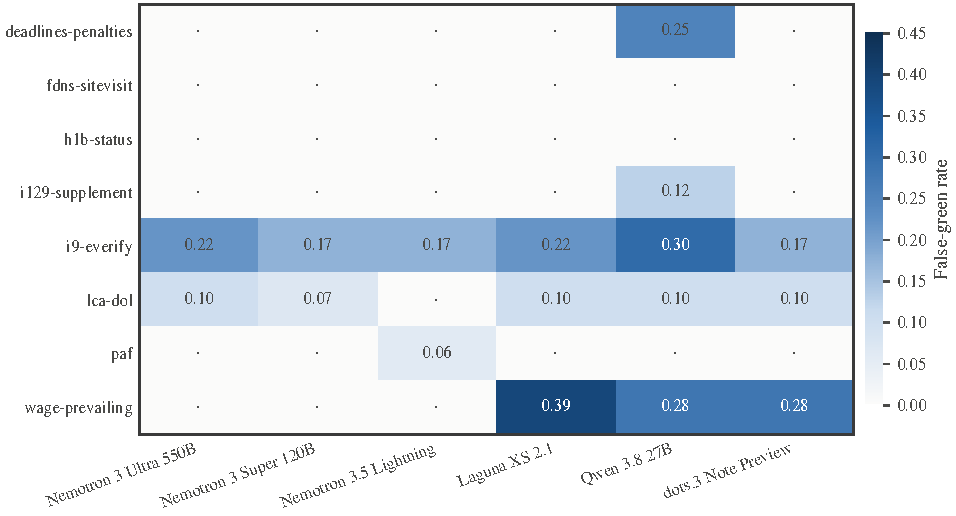
\includegraphics[width=\textwidth]{figures/fig_regime_heatmap.pdf}
\caption{False-green rate by regime and model on the anchor subset, offered schema (the data of Table 13). False greens concentrate in the regimes whose exports carry a populated column next to the missing evidence.}\label{fig:fig_regime_heatmap}
\end{figure}

\subsection{Further declared analyses}\label{sec:D.5}
\textbf{Which failure dominates.} Offered an abstention, each model misses between 11 and 19 of the 20 violation labels (counting unanswered pairs as misses) and reports 5 to 17 of the 120 withheld pairs as compliant, so as a rate the missed violation is the larger failure for every model. No reply line named a pair without a verdict; formatting failures were whole replies with no usable lines, which appear as unanswered pairs (48 and 72 in Lightning's two runs, 16 and 12 in Laguna's). Without the abstention each model misses 1 to 10 violations, and most unassessable pairs become unsupported violations (32 to 99 of 120) or false greens (21 to 63): the withheld condition buys recall by calling unassessable pairs violations.

\textbf{Where abstention is hardest.} The declared hypothesis was that obligations whose evidence is a \emph{document} (a posting notice, a public access file) show more false greens than those whose evidence is a \emph{field} (an I-94 expiry), because a missing document is visible only as a record never expected to exist. Classes were assigned mechanically from each obligation's ``information needed'' text, committed before any rate was computed by class: 49 document and 71 field pairs among the 120 withheld (\texttt{\path|docs/evidence_class_assignment.txt|}). \emph{Result:} in 11 of the 12 runs the document rate is higher. Under \texttt{\path|abstain_offered|} the totals across models are 25 false greens in 426 field-pair evaluations against 38 in 294 document-pair evaluations, about 0.06 against 0.13; the runs share pairs, so we report counts and direction, not a p-value. The one exception, Lightning without the abstention, holds even among pairs it answered (0.575 on field pairs against 0.118 on document pairs).

\textbf{Qualitative failure cases.} To keep excerpts from being the worst lines picked out of thousands, the rule was fixed in code before any was read: for each model, under \texttt{\path|abstain_offered|}, the first \texttt{\path|pass|} on a withheld pair whose reply cites an evidence field. Applied as declared, it selected the same line for four of the six free models: a \texttt{\path|pass|} on the Section 2 employer signature citing \texttt{\path|section2_signed_date|}, the label the audit later overturned. Four models independently reading a populated signed-date column as a signature suggests the label was at fault (D.3), and the prompt's own example of matching columns by meaning names that column. Applying the rule again while skipping overturned pairs, a step added after the first result was seen, gives the excerpts in Section 7.

\section{Study 2, six generated firms without proxy columns}\label{app:E}
Study 2 runs the same protocol on all 252 pairs of six generated firms (Section 4.2), which carry what the anchor firm lacks: conforming controls, a third of them near-miss cases on the legal boundary. Firms were fixed in \texttt{\path|nofalsegreen/study2.py|} before any call. Results come from the three repeated-run models, three runs each, in the Study 2 rows of Table 15. The declared free-tier sweep was stopped after one model, superseded by Study 3 (Section 6), which runs four models from other developers on fresh firms.

\textbf{A scoping defect, and what it touches.} While preparing Study 3 we found that the scoped prompt for the wage rule never carried a generated firm's \texttt{\path|actual_wage_system|} export, which the rule needs. In Study 2 every wage pair was therefore sent without it. The 27 withheld wage pairs are unaffected, since their evidence was missing either way. The 27 decidable wage pairs (three firms, labelled \texttt{\path|pass|} or \texttt{\path|fail|}) were not decidable from what the models saw, and are excluded from every Study 2 metric. False-green rates and the Table 16 contrasts do not change. Detection and false-alarm figures do, and one reading in an earlier version of this paper was wrong: we attributed Gemini 3.1 Pro's near-miss false alarms (0.162) to caution about evidence that was present. They were requests for the missing actual-wage export, which was correct. The defect is fixed for Study 3.

\textbf{Schema contrasts.} On these firms no contrast survives correction (Table 16), consistent with firms that carry no proxy columns.

\textbf{Generated firms are easier.} With abstention offered, the three models report 0.021 to 0.071 of unassessable pairs as compliant, below their anchor-firm rates. Gemini 3.1 Pro and 3.8 Flash detect every violation and raise no false alarm on a conforming control, near-miss controls included, in three of the four schemas. Gemma 4 detects 0.346 of violations and, with abstention offered, raises 0.074 near-miss false alarms. The generated exports are clean, with no populated column next to a missing one, which is the gap Study 3 fills. Excluding the reverification pairs, whose violation labels assume no extension was filed (Section 9), changes no conclusion; no false green fell on them.

\section{Study 3 details and repeated-run tables}\label{app:F}
\begin{figure*}[t]\centering
\begin{adjustbox}{max width=\textwidth}{\scriptsize\ttfamily\setlength{\tabcolsep}{3pt}\renewcommand{\arraystretch}{1.15}%
\begin{tabular}{@{}l@{\hspace{10pt}}l@{}}
\multicolumn{2}{@{}l}{\normalfont\footnotesize\textbf{hris\_roster\_export.csv} \normalfont\footnotesize(first two workers; seed 1018, which withholds \texttt{i9\_record\_export})}\\[2pt]
\textnormal{\footnotesize\textit{Plain}} &
\begin{tabular}{llllll}
\toprule
employeeNumber & visaType & jobTitle & hireDate & employmentStatus & \ldots\\
\midrule
SYN-1001 & H-1B & Computer Systems Analysts & 2024-11-05 & Active & \\
SYN-1002 & H-1B & Computer Systems Analysts & 2022-02-03 & Active & \\
\bottomrule
\end{tabular}\\[16pt]
\textnormal{\footnotesize\textit{Proxy}} &
\begin{tabular}{llll>{\columncolor{fgorange!14}}l>{\columncolor{fgorange!14}}l>{\columncolor{fgorange!14}}l>{\columncolor{fgorange!14}}l>{\columncolor{fgorange!14}}l}
\toprule
employeeNumber & visaType & hireDate & \ldots & i9Status & onboardingCompletedDate & workAuthValidThrough & annualBaseSalary & payBandMidpoint\\
\midrule
SYN-1001 & H-1B & 2024-11-05 & & Complete & 2024-11-02 & 2027-04-29 & 118800 & 106800\\
SYN-1002 & H-1B & 2022-02-03 & & Complete & 2022-01-30 & 2028-11-05 & 118800 & 108000\\
\bottomrule
\end{tabular}
\end{tabular}}
\end{adjustbox}
\caption{Study 3 firm 1018 as generated, rendered plain and with proxy columns. Both withhold the I-9 export, so every I-9 pair is unassessable in both; the proxy rendering adds five roster columns (shaded); every label and every other export is identical. }\label{fig:fig_proxy}
\end{figure*}

\begin{figure}[t]\centering
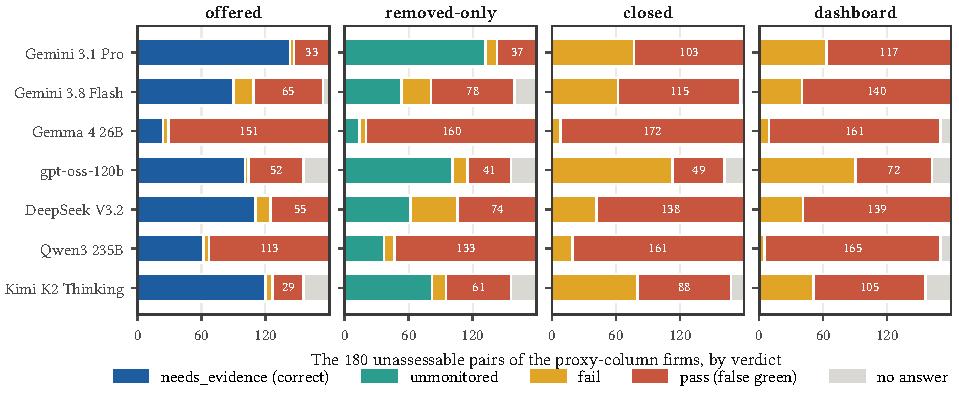
\includegraphics[width=\textwidth]{figures/fig_verdict_flow.pdf}
\caption{Study 3, proxy-column firms: where the 180 unassessable pairs go under each schema. Removing needs\_evidence alone sends many pairs to unmonitored; removing every non-committal verdict sends them to fail or pass, in proportions that differ by model.}\label{fig:fig_verdict_flow}
\end{figure}

\begin{figure}[t]\centering
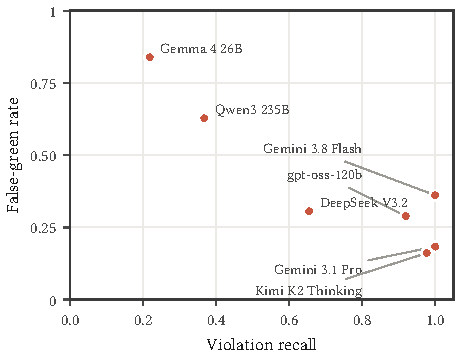
\includegraphics[width=0.5\textwidth]{figures/fig_detection_vs_safety.pdf}
\caption{Study 3, proxy-column firms, offered schema: violation recall against false-green rate, one point per model. Higher recall goes with fewer false greens (Spearman −0.55), but no high-recall model is near zero.}\label{fig:fig_detection_vs_safety}
\end{figure}

\begin{table}[t]
\centering\footnotesize\setlength{\tabcolsep}{4pt}
\caption{Schema contrasts on plain and proxy-column firms (exploratory).}
\label{tab:14}
\begin{adjustbox}{max width=\textwidth}
\begin{tabular}{lrr}
\toprule
\textbf{Change of schema} & \textbf{Plain firms (exploratory)} & \textbf{Proxy firms (declared test)} \\
\midrule
Abstention: offered → closed & +0.093 [+0.04, +0.16], p < 0.001 unadjusted & +0.259 [+0.20, +0.33], Holm p = 0.002 \\
Definition and warning: closed → dashboard & +0.035 [+0.01, +0.06], p = 0.008 unadjusted & +0.084 [+0.04, +0.12], Holm p = 0.002 \\
\bottomrule
\end{tabular}
\end{adjustbox}
\par\vspace{3pt}\begin{minipage}{\textwidth}\scriptsize Pooled over the seven models with equal weight; same pairs, clusters and bootstrap draws as the declared analysis. The plain-firm column was computed after the results and is not part of any declared family.\end{minipage}
\end{table}

\begin{sidewaystable}
\centering\footnotesize\setlength{\tabcolsep}{4pt}
\caption{The three repeated-run models, both studies, four schemas. Mean of three runs, with the minimum and maximum in brackets.}
\label{tab:15}
\begin{adjustbox}{max width=\textheight}
\begin{tabular}{lrlrrrlrr}
\toprule
\textbf{Model} & \textbf{Study} & \textbf{Schema} & \textbf{False green} & \textbf{FG, answered only} & \textbf{Recall} & \textbf{False alarm, near-miss} & \textbf{Unassessable pairs answered pass / fail / needs\_ev. / unmon.} & \textbf{Min answered} \\
\midrule
Gemini 3.1 Pro & 1 & offered & 0.058 [0.058, 0.058] & 0.058 & 0.433 [0.400, 0.450] & — & 7 / 1 / 101 / 11 & 140/140 \\
Gemini 3.1 Pro & 1 & removed-only & 0.050 [0.025, 0.067] & 0.050 & 0.550 [0.500, 0.600] & — & 6 / 5 / 0 / 109 & 140/140 \\
Gemini 3.1 Pro & 1 & closed & 0.050 [0.033, 0.067] & 0.050 & 0.950 [0.950, 0.950] & — & 6 / 114 / 0 / 0 & 140/140 \\
Gemini 3.1 Pro & 1 & dashboard & 0.131 [0.125, 0.142] & 0.131 & 0.917 [0.850, 0.950] & — & 16 / 104 / 0 / 0 & 140/140 \\
Gemini 3.1 Pro & 2 & offered & 0.021 [0.016, 0.032] & 0.021 & 1.000 [1.000, 1.000] & 0.000 [0.000, 0.000] & 3 / 0 / 123 / 0 & 225/252 \\
Gemini 3.1 Pro & 2 & removed-only & 0.056 [0.024, 0.071] & 0.056 & 1.000 [1.000, 1.000] & 0.025 [0.000, 0.037] & 7 / 26 / 0 / 93 & 225/252 \\
Gemini 3.1 Pro & 2 & closed & 0.061 [0.056, 0.064] & 0.061 & 1.000 [1.000, 1.000] & 0.000 [0.000, 0.000] & 8 / 118 / 0 / 0 & 225/252 \\
Gemini 3.1 Pro & 2 & dashboard & 0.061 [0.056, 0.064] & 0.061 & 1.000 [1.000, 1.000] & 0.000 [0.000, 0.000] & 8 / 118 / 0 / 0 & 225/252 \\
Gemini 3.8 Flash & 1 & offered & 0.094 [0.092, 0.100] & 0.094 & 0.500 [0.500, 0.500] & — & 11 / 0 / 96 / 12 & 140/140 \\
Gemini 3.8 Flash & 1 & removed-only & 0.156 [0.125, 0.183] & 0.160 & 0.783 [0.750, 0.850] & — & 19 / 18 / 0 / 79 & 128/140 \\
Gemini 3.8 Flash & 1 & closed & 0.242 [0.208, 0.283] & 0.245 & 0.767 [0.600, 0.850] & — & 29 / 89 / 0 / 0 & 127/140 \\
Gemini 3.8 Flash & 1 & dashboard & 0.419 [0.375, 0.458] & 0.433 & 0.833 [0.800, 0.850] & — & 50 / 66 / 0 / 0 & 127/140 \\
Gemini 3.8 Flash & 2 & offered & 0.026 [0.016, 0.032] & 0.027 & 1.000 [1.000, 1.000] & 0.000 [0.000, 0.000] & 3 / 4 / 117 / 0 & 219/252 \\
Gemini 3.8 Flash & 2 & removed-only & 0.037 [0.032, 0.048] & 0.037 & 1.000 [1.000, 1.000] & 0.000 [0.000, 0.000] & 5 / 62 / 0 / 59 & 225/252 \\
Gemini 3.8 Flash & 2 & closed & 0.156 [0.127, 0.182] & 0.156 & 1.000 [1.000, 1.000] & 0.000 [0.000, 0.000] & 20 / 106 / 0 / 0 & 225/252 \\
Gemini 3.8 Flash & 2 & dashboard & 0.167 [0.167, 0.167] & 0.167 & 1.000 [1.000, 1.000] & 0.000 [0.000, 0.000] & 21 / 105 / 0 / 0 & 225/252 \\
Gemma 4 26B & 1 & offered & 0.153 [0.150, 0.158] & 0.153 & 0.067 [0.050, 0.100] & — & 18 / 0 / 76 / 26 & 140/140 \\
Gemma 4 26B & 1 & removed-only & 0.183 [0.175, 0.200] & 0.220 & 0.067 [0.050, 0.100] & — & 22 / 0 / 0 / 79 & 116/140 \\
Gemma 4 26B & 1 & closed & 0.600 [0.525, 0.667] & 0.682 & 0.400 [0.400, 0.400] & — & 72 / 33 / 0 / 0 & 122/140 \\
Gemma 4 26B & 1 & dashboard & 0.589 [0.567, 0.617] & 0.635 & 0.400 [0.400, 0.400] & — & 71 / 41 / 0 / 0 & 128/140 \\
Gemma 4 26B & 2 & offered & 0.071 [0.071, 0.071] & 0.071 & 0.346 [0.296, 0.370] & 0.074 [0.074, 0.074] & 9 / 0 / 116 / 1 & 225/252 \\
Gemma 4 26B & 2 & removed-only & 0.071 [0.071, 0.071] & 0.071 & 0.370 [0.333, 0.407] & 0.111 [0.111, 0.111] & 9 / 0 / 0 / 117 & 225/252 \\
Gemma 4 26B & 2 & closed & 0.172 [0.167, 0.175] & 0.189 & 0.444 [0.370, 0.518] & 0.049 [0.037, 0.074] & 22 / 93 / 0 / 0 & 208/252 \\
Gemma 4 26B & 2 & dashboard & 0.175 [0.175, 0.175] & 0.175 & 0.370 [0.370, 0.370] & 0.037 [0.037, 0.037] & 22 / 104 / 0 / 0 & 225/252 \\
\bottomrule
\end{tabular}
\end{adjustbox}
\par\vspace{3pt}\begin{minipage}{\textheight}\scriptsize Schemas: \emph{offered} (four verdicts, evidence-anchored definitions); \emph{removed-only} (offered minus \texttt{needs\_\allowbreak{}evidence}); \emph{closed} (\texttt{pass}/\texttt{fail} only, evidence-anchored definitions kept); \emph{dashboard} (\texttt{pass}/\texttt{fail} only, \texttt{pass} redefined as ``the obligation is satisfied'', warning dropped). The anchor subset has 120 unassessable pairs and no controls; Study 2 rates are pooled over its six firms (126 unassessable pairs). Min answered: the fewest pairs answered in any of the three runs. The verdict columns show every off-schema answer: none occurred on an unassessable pair in any cell.\end{minipage}
\end{sidewaystable}

\begin{table}[t]
\centering\footnotesize\setlength{\tabcolsep}{4pt}
\caption{Paired schema contrasts, repeated-run models.}
\label{tab:16}
\begin{adjustbox}{max width=\textwidth}
\begin{tabular}{lrlrrr}
\toprule
\textbf{Model} & \textbf{Study} & \textbf{Change of schema} & \textbf{Unassessable pairs} & \textbf{Change in FGR [95\% CI]} & \textbf{Holm p} \\
\midrule
Gemini 3.1 Pro & 1 & offered → removed-only & 120 & -0.008 [-0.04, +0.01] & 1.000 \\
Gemini 3.1 Pro & 1 & offered → closed & 120 & -0.008 [-0.09, +0.05] & 1.000 \\
Gemini 3.1 Pro & 1 & closed → dashboard & 120 & +0.081 [+0.02, +0.17] & 0.036 ** \\
Gemini 3.1 Pro & 1 & offered → dashboard & 120 & +0.072 [-0.04, +0.19] & 1.000 \\
Gemini 3.1 Pro & 2 & offered → removed-only & 126 & +0.034 [+0.00, +0.11] & 1.000 \\
Gemini 3.1 Pro & 2 & offered → closed & 126 & +0.040 [+0.00, +0.10] & 1.000 \\
Gemini 3.1 Pro & 2 & closed → dashboard & 126 & +0.000 [+0.00, +0.00] & 1.000 \\
Gemini 3.1 Pro & 2 & offered → dashboard & 126 & +0.040 [+0.00, +0.10] & 1.000 \\
Gemini 3.8 Flash & 1 & offered → removed-only & 108 & +0.077 [-0.01, +0.20] & 1.000 \\
Gemini 3.8 Flash & 1 & offered → closed & 115 & +0.136 [+0.04, +0.24] & 0.019 ** \\
Gemini 3.8 Flash & 1 & closed → dashboard & 103 & +0.168 [+0.10, +0.24] & 0.012 ** \\
Gemini 3.8 Flash & 1 & offered → dashboard & 108 & +0.324 [+0.17, +0.48] & 0.012 ** \\
Gemini 3.8 Flash & 2 & offered → removed-only & 120 & +0.003 [+0.00, +0.01] & 1.000 \\
Gemini 3.8 Flash & 2 & offered → closed & 120 & +0.133 [+0.00, +0.33] & 0.960 \\
Gemini 3.8 Flash & 2 & closed → dashboard & 126 & +0.011 [-0.01, +0.04] & 1.000 \\
Gemini 3.8 Flash & 2 & offered → dashboard & 120 & +0.142 [+0.00, +0.37] & 1.000 \\
Gemma 4 26B & 1 & offered → removed-only & 97 & +0.086 [+0.01, +0.20] & 0.012 ** \\
Gemma 4 26B & 1 & offered → closed & 102 & +0.542 [+0.38, +0.70] & 0.012 ** \\
Gemma 4 26B & 1 & closed → dashboard & 102 & -0.049 [-0.16, +0.04] & 1.000 \\
Gemma 4 26B & 1 & offered → dashboard & 108 & +0.509 [+0.34, +0.67] & 0.012 ** \\
Gemma 4 26B & 2 & offered → removed-only & 126 & +0.000 [+0.00, +0.00] & 1.000 \\
Gemma 4 26B & 2 & offered → closed & 109 & +0.110 [+0.01, +0.25] & 0.320 \\
Gemma 4 26B & 2 & closed → dashboard & 109 & +0.000 [+0.00, +0.00] & 1.000 \\
Gemma 4 26B & 2 & offered → dashboard & 126 & +0.103 [+0.02, +0.24] & 0.102 \\
\bottomrule
\end{tabular}
\end{adjustbox}
\par\vspace{3pt}\begin{minipage}{\textwidth}\scriptsize Each unassessable pair's outcome is its share of \texttt{pass} over the three runs. Pairs answered in every run of both conditions; obligations resampled (2,000 draws, firm by obligation in Study 2); two-sided p-values Holm-corrected across all 24 contrasts; ** marks p < 0.05.\end{minipage}
\end{table}

\textbf{Repeats are close.} Across the 24 model, study and schema cells, the three runs' false-green rates differ by at most 0.142, and by 0.06 or less in 21 of them. That bounds run-to-run variation on one host at temperature 0; it says nothing about variation across hosts, so it does not license the single runs of Section 7.

\begin{table}[t]
\centering\footnotesize\setlength{\tabcolsep}{4pt}
\caption{Study 3, false-green rate by model, firm rendering and schema.}
\label{tab:17}
\begin{adjustbox}{max width=\textwidth}
\begin{tabular}{llrrrrrrr}
\toprule
\textbf{Model} & \textbf{Arm} & \textbf{FGR offered} & \textbf{removed-only} & \textbf{closed} & \textbf{dashboard} & \textbf{Recall, offered} & \textbf{False alarm, offered} & \textbf{Min answered} \\
\midrule
Gemini 3.1 Pro & plain & 0.106 & 0.189 & 0.206 & 0.294 & 1.000 & 0.000 & 504/504 \\
Gemini 3.1 Pro & proxy & 0.183 & 0.206 & 0.572 & 0.650 & 1.000 & 0.000 & 504/504 \\
Gemini 3.8 Flash & plain & 0.161 & 0.217 & 0.350 & 0.361 & 1.000 & 0.000 & 498/504 \\
Gemini 3.8 Flash & proxy & 0.361 & 0.433 & 0.639 & 0.778 & 1.000 & 0.000 & 471/504 \\
Gemma 4 26B & plain & 0.339 & 0.333 & 0.406 & 0.411 & 0.230 & 0.084 & 498/504 \\
Gemma 4 26B & proxy & 0.839 & 0.889 & 0.956 & 0.894 & 0.218 & 0.093 & 494/504 \\
gpt-oss-120b & plain & 0.133 & 0.239 & 0.228 & 0.228 & 0.954 & 0.017 & 474/504 \\
gpt-oss-120b & proxy & 0.289 & 0.228 & 0.272 & 0.400 & 0.920 & 0.030 & 468/504 \\
DeepSeek V3.2 & plain & 0.111 & 0.211 & 0.189 & 0.267 & 0.529 & 0.131 & 504/504 \\
DeepSeek V3.2 & proxy & 0.306 & 0.411 & 0.767 & 0.772 & 0.655 & 0.127 & 504/504 \\
Qwen3 235B & plain & 0.317 & 0.350 & 0.367 & 0.394 & 0.345 & 0.194 & 489/504 \\
Qwen3 235B & proxy & 0.628 & 0.739 & 0.894 & 0.917 & 0.368 & 0.232 & 494/504 \\
Kimi K2 Thinking & plain & 0.156 & 0.161 & 0.261 & 0.233 & 0.966 & 0.000 & 474/504 \\
Kimi K2 Thinking & proxy & 0.161 & 0.339 & 0.489 & 0.583 & 0.977 & 0.034 & 456/504 \\
\bottomrule
\end{tabular}
\end{adjustbox}
\par\vspace{3pt}\begin{minipage}{\textwidth}\scriptsize Twelve fresh firms (504 pairs, 180 unassessable) per arm, one run per cell. \emph{plain}: generator v2; \emph{proxy}: the same firms with the five proxy columns (generator v3). False alarm is any non-\texttt{pass} verdict on one of the 237 conforming controls.\end{minipage}
\end{table}

\begin{sidewaystable}
\centering\footnotesize\setlength{\tabcolsep}{4pt}
\caption{Study 3, the declared tests.}
\label{tab:18}
\begin{adjustbox}{max width=\textheight}
\begin{tabular}{lrrrr}
\toprule
\textbf{Estimate} & \textbf{P1 abstention} & \textbf{P2 definition and warning} & \textbf{P3 proxy columns, dashboard} & \textbf{P4 proxy columns, offered} \\
\midrule
\textbf{Pooled, 7 models (primary)} & +0.259 [+0.20, +0.33] p=0.002 ** & +0.084 [+0.04, +0.12] p=0.002 ** & +0.427 [+0.29, +0.56] p=0.002 ** & +0.217 [+0.15, +0.29] p=0.002 ** \\
Google, 3 models & +0.258 [+0.16, +0.36] p=0.004 ** & +0.069 [+0.01, +0.13] p=0.021 ** & +0.440 [+0.27, +0.61] p=0.004 ** & +0.265 [+0.18, +0.35] p=0.004 ** \\
Other developers, 4 models & +0.260 [+0.18, +0.34] p=0.004 ** & +0.095 [+0.04, +0.14] p=0.004 ** & +0.417 [+0.29, +0.53] p=0.004 ** & +0.181 [+0.12, +0.26] p=0.004 ** \\
Gemini 3.1 Pro & +0.389 [+0.24, +0.55] p=0.014 ** & +0.078 [+0.00, +0.17] p=0.432 & +0.356 [+0.22, +0.50] p=0.014 ** & +0.078 [+0.01, +0.17] p=0.432 \\
Gemini 3.8 Flash & +0.269 [+0.10, +0.46] p=0.014 ** & +0.136 [+0.00, +0.27] p=0.432 & +0.417 [+0.18, +0.64] p=0.015 ** & +0.218 [+0.07, +0.40] p=0.033 ** \\
Gemma 4 26B & +0.117 [+0.00, +0.25] p=0.432 & -0.006 [-0.02, +0.00] p=1.000 & +0.547 [+0.34, +0.72] p=0.014 ** & +0.500 [+0.29, +0.69] p=0.014 ** \\
gpt-oss-120b & -0.020 [-0.12, +0.07] p=1.000 & +0.154 [+0.07, +0.23] p=0.014 ** & +0.174 [+0.08, +0.25] p=0.014 ** & +0.160 [+0.05, +0.30] p=0.015 ** \\
DeepSeek V3.2 & +0.461 [+0.28, +0.62] p=0.014 ** & +0.006 [-0.06, +0.07] p=1.000 & +0.506 [+0.35, +0.66] p=0.014 ** & +0.194 [+0.06, +0.36] p=0.015 ** \\
Qwen3 235B & +0.267 [+0.12, +0.40] p=0.014 ** & +0.035 [-0.04, +0.11] p=1.000 & +0.545 [+0.32, +0.74] p=0.014 ** & +0.311 [+0.19, +0.45] p=0.014 ** \\
Kimi K2 Thinking & +0.333 [+0.20, +0.49] p=0.014 ** & +0.187 [+0.06, +0.31] p=0.070 & +0.444 [+0.25, +0.63] p=0.015 ** & +0.058 [-0.03, +0.17] p=1.000 \\
\bottomrule
\end{tabular}
\end{adjustbox}
\par\vspace{3pt}\begin{minipage}{\textheight}\scriptsize Difference in false-green rate on unassessable pairs answered in both cells, [95\% CI] from an obligation-cluster bootstrap (18 firm-by-rule clusters, 2,000 draws), Holm-adjusted p. Holm families as declared: the four pooled tests; the 28 per-model tests; the eight group tests. ** marks adjusted p < 0.05. Pooled estimates weight each model equally.\end{minipage}
\end{sidewaystable}

\begin{table}[t]
\centering\footnotesize\setlength{\tabcolsep}{4pt}
\caption{Per-model effects of the declared tests of Studies 4–7.}
\label{tab:19}
\begin{adjustbox}{max width=\textwidth}
\begin{tabular}{lrrrrr}
\toprule
\textbf{Test} & \textbf{Gemini 3.1 Pro} & \textbf{Gemini 3.8 Flash} & \textbf{Gemma 4 26B} & \textbf{DeepSeek V3.2} & \textbf{GLM-5.2} \\
\midrule
H1 Names & +0.021 & +0.115 & +0.612 & +0.091 & -0.091 \\
H2 Meaning & +0.021 & +0.115 & +0.758 & +0.121 & +0.115 \\
H3 Direction (\texttt{fail}) & +0.000 & +0.000 & +0.076 & +0.076 & +0.051 \\
H4 Abstaining verdicts & +0.519 & +0.444 & +0.188 & +0.564 & +0.725 \\
H5 Bare definitions & -0.087 & +0.001 & -0.027 & +0.045 & +0.068 \\
H6 Warning & +0.166 & +0.114 & -0.003 & +0.059 & -0.005 \\
H7 Evidence-first prompt & +0.021 & +0.067 & +0.133 & +0.106 & +0.088 \\
R1 Pay fields, offered & +0.000 & +0.496 & +0.182 & +0.748 & +0.382 \\
R2 Pay fields, dashboard & +0.325 & +0.000 & +0.000 & +0.092 & +0.000 \\
R3 Dashboard − offered & +0.583 & +1.000 & +0.175 & +0.783 & +1.000 \\
W1 Pay Rate alone & +0.000 & +0.160 & +0.182 & +0.775 & +0.000 \\
W2 Pay type and schedule & +0.000 & +0.000 & +0.175 & +0.158 & +0.000 \\
\bottomrule
\end{tabular}
\end{adjustbox}
\par\vspace{3pt}\begin{minipage}{\textwidth}\scriptsize Each model's effect on the false-green rate (H3: on \texttt{fail}), paired on pairs answered in both cells and pooled over firms; descriptive, computed after the results. Tests in Tables 5 and 6 and Section 6.8.\end{minipage}
\end{table}

\section{Interpretive choices of the reference checker}\label{app:G}
The checker of Section 4.3 records every choice the regulations leave open, with its source, in \texttt{\path|labelcheck/INTERPRETATIONS.md|}. The choices that matter most are these. Section 1 signed on the first day of employment is timely (8 C.F.R. 274a.2(b)(1)(i)(A); M-274 §3.0). Section 2 is due by the third business day after the first day, with weekends and federal holidays (with their observed dates) excluded; the M-274 does not define ``business day''. Reverification on the expiry date itself is timely. The required wage is the greater of the prevailing wage and the actual wage, compared per pay period rather than as a year-to-date average (20 C.F.R. 655.731(a), (c)(4)). None of the five proxy columns is treated as evidence. Section 4.3 gives the number of verdicts each boundary choice would change.

Across the checked firms, 70 Section 2 dates fall exactly on the deadline day; counting weekdays without excluding federal holidays would change 6 verdicts, and counting calendar days 55. The 1,176 distinct labels are 1,680 counting the proxy twins of Study 3, whose labels are identical by construction (\texttt{\path|docs/labelcheck_results.json|}).

\section{The same error in a rule engine}\label{app:H}
The defects below were found and fixed in the private repository of the engine that the rulebook comes from (Settle AI Inc.), between 2026-06-28 and 2026-07-14. Commit identifiers are given for the record; the repository is not public. In each case the engine returned a verdict that the available record could not support.

\begin{table}[t]
\centering\footnotesize\setlength{\tabcolsep}{4pt}
\begin{tabularx}{\textwidth}{>{\raggedright\arraybackslash}X>{\raggedright\arraybackslash}X>{\raggedright\arraybackslash}X}
\toprule
\textbf{Defect} & \textbf{What the code did} & \textbf{Fix} \\
\midrule
Silent skip, I-9 Section 2 and reverification & An evaluator skipped an employee whose record lacked the deciding dates, so the employee left monitoring and the dashboard stayed green & Emit a visible \texttt{needs\_\allowbreak{}evidence} finding (commits \texttt{16de553c}, \texttt{407eb438}; an internal review note calls it ``a verified production defect'') \\
Salary of record as wages paid & The material-change wage check returned pass or fail from the HR salary of record & Retired: a salary of record ``proves nothing about wages paid''; it never passes alone (commits \texttt{1b181e00}, \texttt{4b2605ec}) \\
Required wage without the actual-wage limb & The greater-of rule passed on the prevailing wage alone when the employer's actual-wage benchmark was unknown & The would-be pass becomes \texttt{needs\_\allowbreak{}evidence} (commit \texttt{55c5e6fb}) \\
Fabricated provenance & Wage cohorts were stamped with a prevailing-wage source and an ``ok'' document status that no input supplied & Stored as unknown, so the rules ask for the record (commit \texttt{c47a945b}) \\
\bottomrule
\end{tabularx}
\end{table}

Because the repository is private, the logic of each defect is restated below as pseudocode (paraphrased, not copied), so that the claim can be checked against the description.

\begin{Verbatim}[breaklines,breakanywhere,fontsize=\scriptsize,frame=single,framerule=0.3pt,rulecolor=\color{fggray}]
# silent skip (I-9 Section 2; reverification)
before: for worker in workers:
            record = i9_records.get(worker)
            if record is None or record.section2_date is None: continue   # worker leaves monitoring
            emit(check(record))
after:      if record is None or record.section2_date is None:
                emit(needs_evidence(worker, missing="Section 2 date")); continue

# salary of record as wages paid
before: verdict = PASS if roster.salary >= lca.required_wage else FAIL
after:  verdict = NEEDS_EVIDENCE unless payroll.periods cover the span; salary alone never passes

# greater-of rule without the actual-wage limb
before: required = lca.prevailing_wage; verdict = PASS if paid >= required else FAIL
after:  if actual_wage_benchmark is None and paid >= lca.prevailing_wage: verdict = NEEDS_EVIDENCE
        else: required = max(lca.prevailing_wage, actual_wage_benchmark); ...

# fabricated provenance
before: cohort.pw_source = "OES"; cohort.pw_doc_status = "ok"
after:  cohort.pw_source = mapped_column or "unknown"   # "unknown" is read as an evidence request
\end{Verbatim}

The engine's rules were written with AI coding assistance, and the defects were found by AI-assisted review (Codex), so the table is not evidence about human engineers. It shows that a system built to fill a dashboard acquires these substitutions easily, and that each fix is the same: return \texttt{\path|needs_evidence|} when the record that decides the obligation is absent.

\section{AI pilot runs of the expert protocol}\label{app:I}
The expert protocol is a workbook of 50 items and 8 statements (\texttt{\path|docs/expert_review_v3/|}, built by \texttt{\path|scripts/build_expert_kit_v3.py|}). Its 50 items are:

\begin{itemize}
\item 20 unassessable pairs on proxy-column firms;
\item 10 unassessable pairs on plain firms;
\item 20 decidable violations and controls, some on the legal boundary.
\end{itemize}

Each item shows the employer's records inline, and the reviewer answers blind to the construction label. No human expert has completed it.

\textbf{What was run.} Two AI systems completed it as a pilot, at the author's request:

\begin{itemize}
\item Claude (Anthropic) completed version 2. Its own answers flagged five defects in the workbook, fixed in version 3: - identifiers repeated across firms; - two items with identical records; - no stated rule on status extensions; - no holiday calendar; - no wage item that could fail.
\item Codex (OpenAI) completed version 3.
\end{itemize}

Both are scored against their own version's labels (\texttt{\path|scripts/score_ai_pilot.py|}, \texttt{\path|docs/ai_pilot_review/results.json|}).

\textbf{Results.} Each agreed with all 50 labels:

\begin{itemize}
\item every proxy-column item was answered \texttt{\path|needs_evidence|};
\item every planted violation was answered \texttt{\path|fail|};
\item every control was answered \texttt{\path|pass|}.
\end{itemize}

On the evidence statements, both strongly disagreed that an I-9 status flag, an onboarding date or a future authorisation end date shows I-9 timeliness, and both strongly disagreed that an LCA's wage shows the wages paid. Both strongly agreed that a missing record should be reported as needing evidence. Claude disagreed, and Codex strongly disagreed, that a salary of record shows the required wage was paid and that an HR status field can mark an item compliant for triage.

\textbf{What this shows.} These runs are not expert validation:

\begin{itemize}
\item \textbf{Not blind to the study.} Both systems worked with the author on this project, and Codex had reviewed earlier drafts of the paper, so neither was blind to the evidence standard.
\item \textbf{Correlated errors.} Systems of the same kind as the models under test may share their errors.
\end{itemize}

The runs show that the protocol can be completed as designed, and that a careful reader of the standard reproduces the labels. Whether practitioners accept that standard remains open (§9).

\end{document}
